
\documentclass[12pt,letterpaper]{article}


\usepackage[utf8]{inputenc}
\usepackage[T1]{fontenc}
\usepackage{amsmath,amssymb}
\usepackage{graphicx}
\usepackage{float}
\usepackage{xcolor}
\usepackage{listings}
\usepackage{enumitem}
\usepackage{hyperref}



\hypersetup{
    pdftitle={Laboratorio 5 ICN-292},
    pdfauthor={Isidora Cordova Stevenson},
    colorlinks=true,
    linkcolor=blue,
    urlcolor=blue,
    citecolor=violet
}



\newcommand{\HRule}{\rule{\linewidth}{0.5mm}}



\lstdefinestyle{sqlstyle}{
    language=SQL,
    basicstyle=\ttfamily\small,
    keywordstyle=\color{blue}\bfseries,
    commentstyle=\color{gray}\itshape,
    stringstyle=\color{teal},
    numberstyle=\tiny\color{gray},
    numbers=left,
    stepnumber=1,
    numbersep=8pt,
    showstringspaces=false,
    breaklines=true,
    breakatwhitespace=false,
    frame=single,
    tabsize=4,
    columns=fullflexible,
    keepspaces=true
}



\begin{document}


\begin{titlepage}
\centering

\includegraphics[scale=.3]{Imagenes/Logo.jpg}

\vspace{12mm}

\textsc{\Large Sistema de Información para la Gestión}\\[0.5cm]

\textit{\large
2do. Semestre 2026 \hspace{5mm}\textbar\hspace{5mm}
Programa Diurno \hspace{5mm}\textbar\hspace{5mm}
Campus Vitacura}\\[0.5cm]

\vspace{8mm}

\HRule \\[6mm]

{\huge \textbf{Informe de Laboratorio 5}}\\[0.4cm]

\HRule \\[10mm]

\begin{minipage}[t]{0.5\textwidth}
\begin{flushleft}
\large
\emph{\textbf{Autora:}}\\
Isidora Renata \textsc{Córdova Stevenson}\\
{\small 202204631-7, Ingeniería Civil Industrial}
\end{flushleft}
\end{minipage}
\hfill
\begin{minipage}[t]{0.4\textwidth}
\begin{flushright}
\large
\emph{\textbf{Profesores:}}\\
Patricio \textsc{Cifuentes}\\
José Luis \textsc{Sáez T.}
\end{flushright}
\end{minipage}\\[12mm]

{\large \textbf{\textit{Enlace Github:}}}\\[1.5mm]

{\small \url{https://github.com/Isiusm/ICN292-Lab5-Cordova-Isidora}}\\[5mm]

\vfill
\end{titlepage}

\section*{Consulta 1}

\begin{lstlisting}[style=sqlstyle]
SELECT ve.nombre,
       COUNT(v.id_venta) AS cantidad_ventas
FROM vendedores ve
LEFT JOIN ventas v
    ON ve.id_vendedor = v.id_vendedor
GROUP BY ve.id_vendedor, ve.nombre
ORDER BY cantidad_ventas DESC, ve.nombre ASC;
\end{lstlisting}

\begin{figure}[H]
\centering
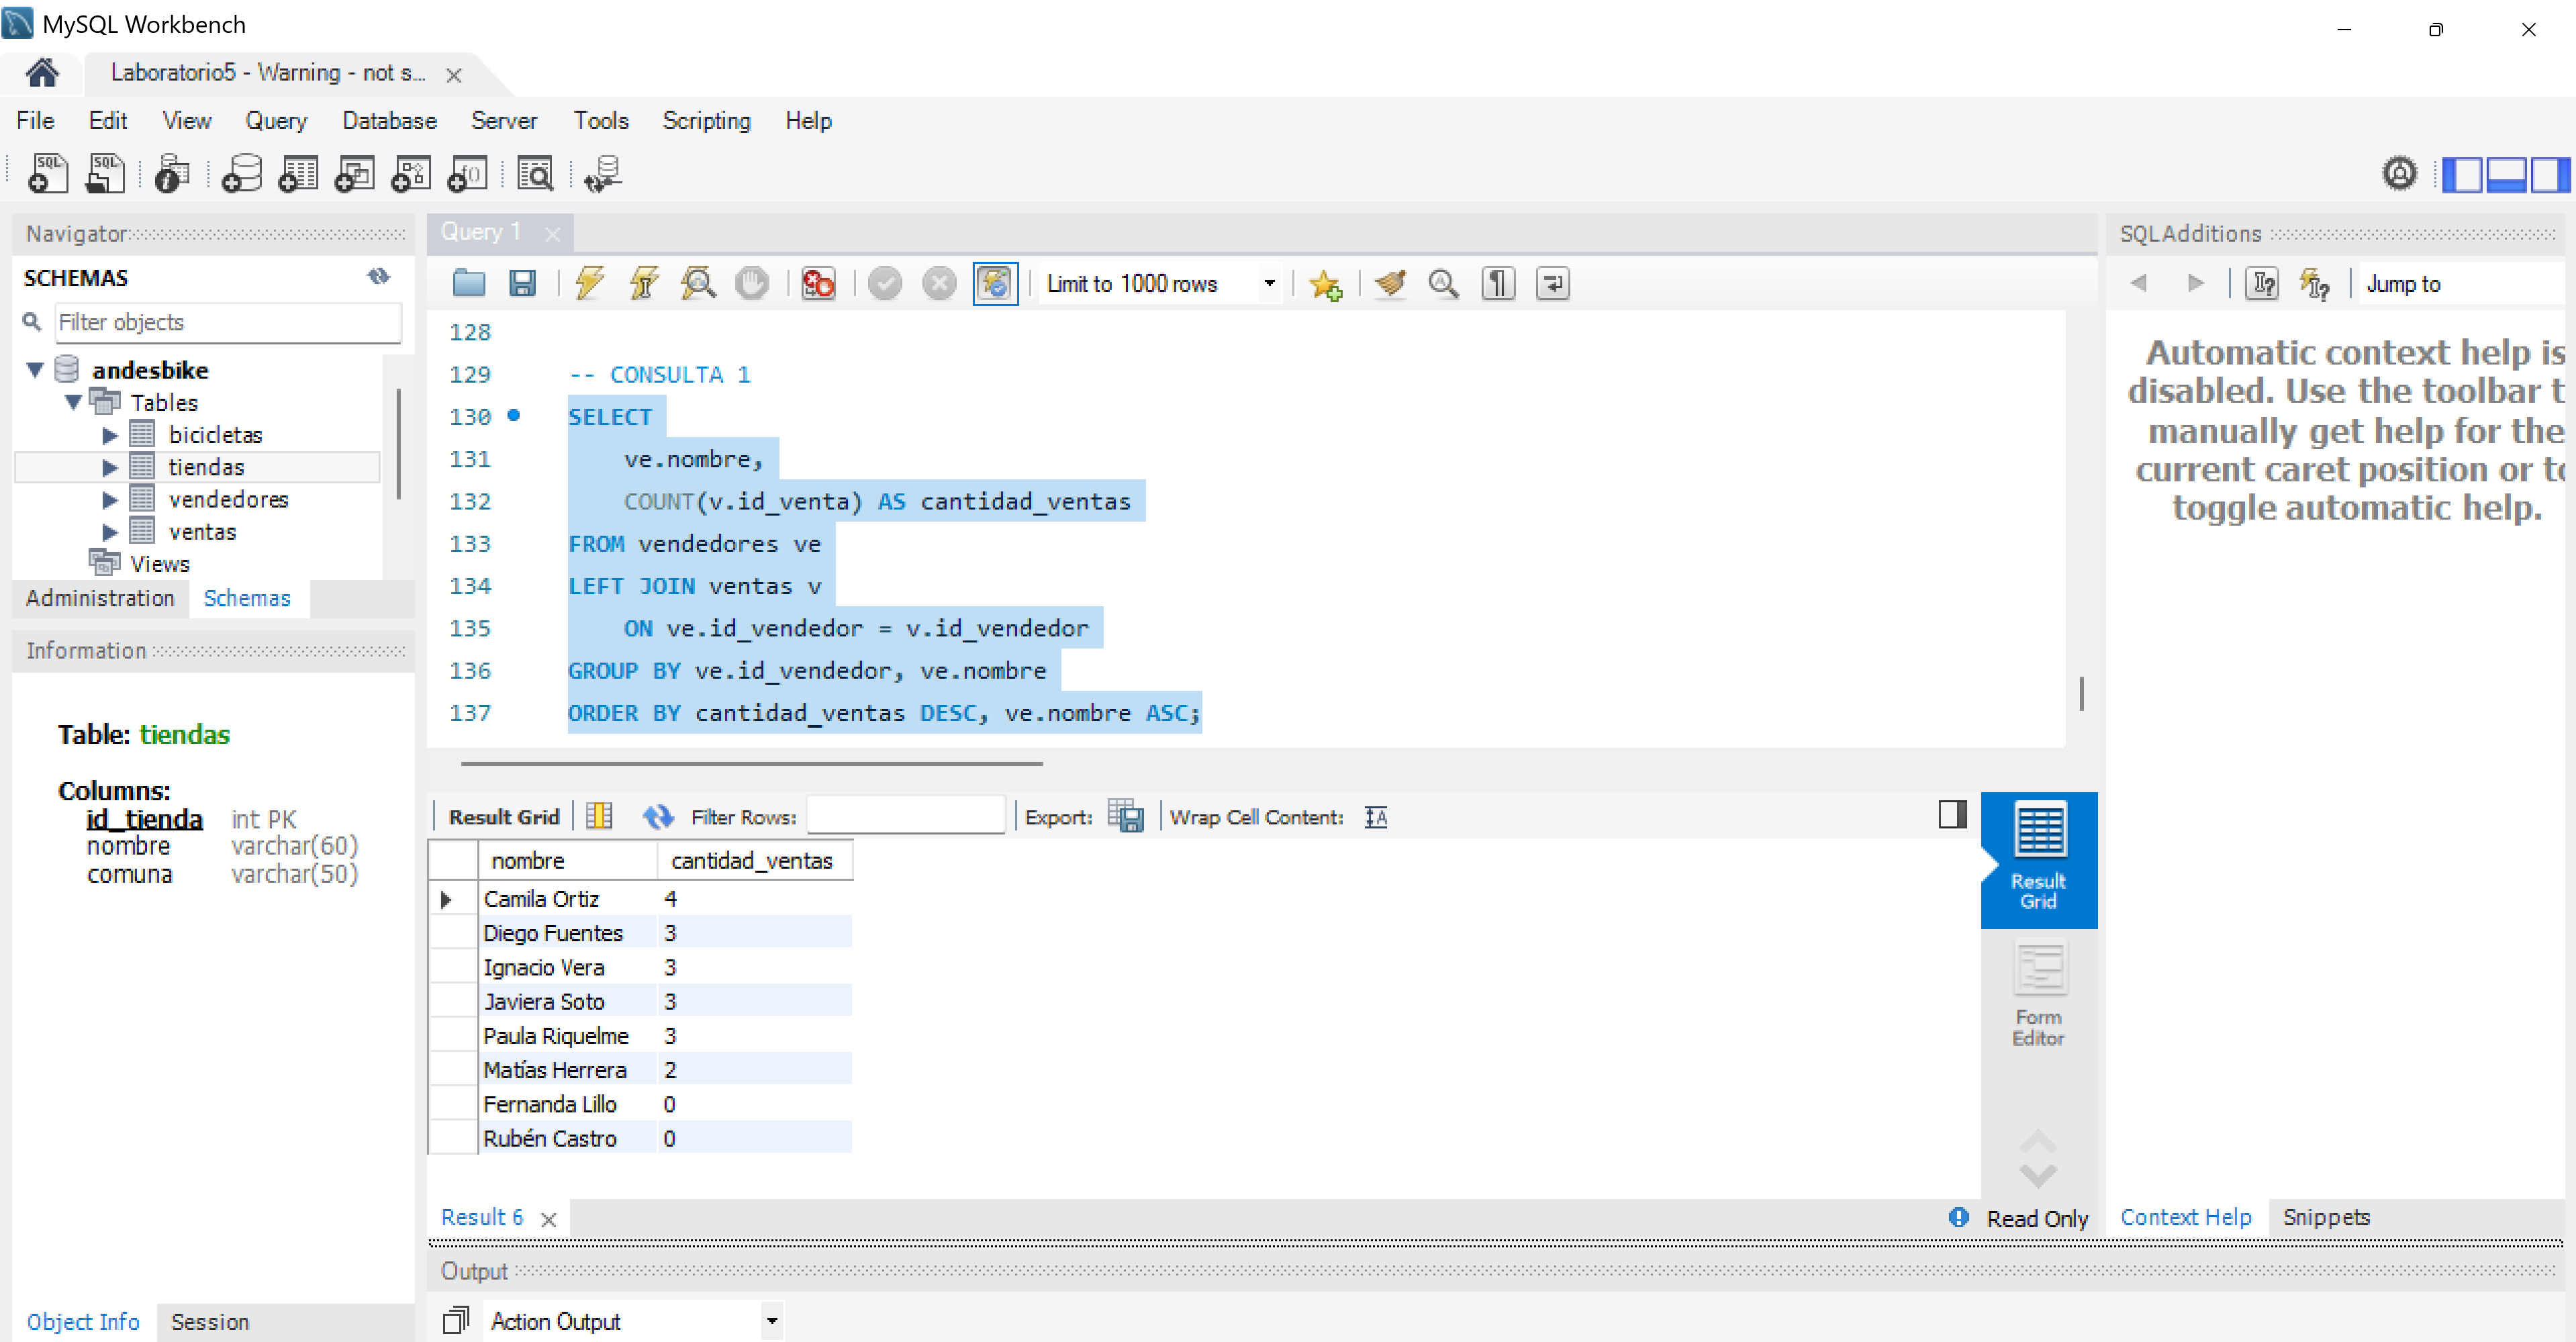
\includegraphics[width=0.95\textwidth,
height=0.38\textheight,keepaspectratio]{Consulta_01.png}
\end{figure}

\clearpage


\section*{Consulta 2}

\begin{lstlisting}[style=sqlstyle]
SELECT t.nombre,
       COUNT(v.id_venta) AS cantidad_ventas,
       COALESCE(SUM(v.unidades), 0) AS unidades_vendidas
FROM tiendas t
LEFT JOIN vendedores ve
    ON t.id_tienda = ve.id_tienda
LEFT JOIN ventas v
    ON ve.id_vendedor = v.id_vendedor
GROUP BY t.id_tienda, t.nombre
ORDER BY unidades_vendidas DESC;
\end{lstlisting}

\begin{figure}[H]
\centering
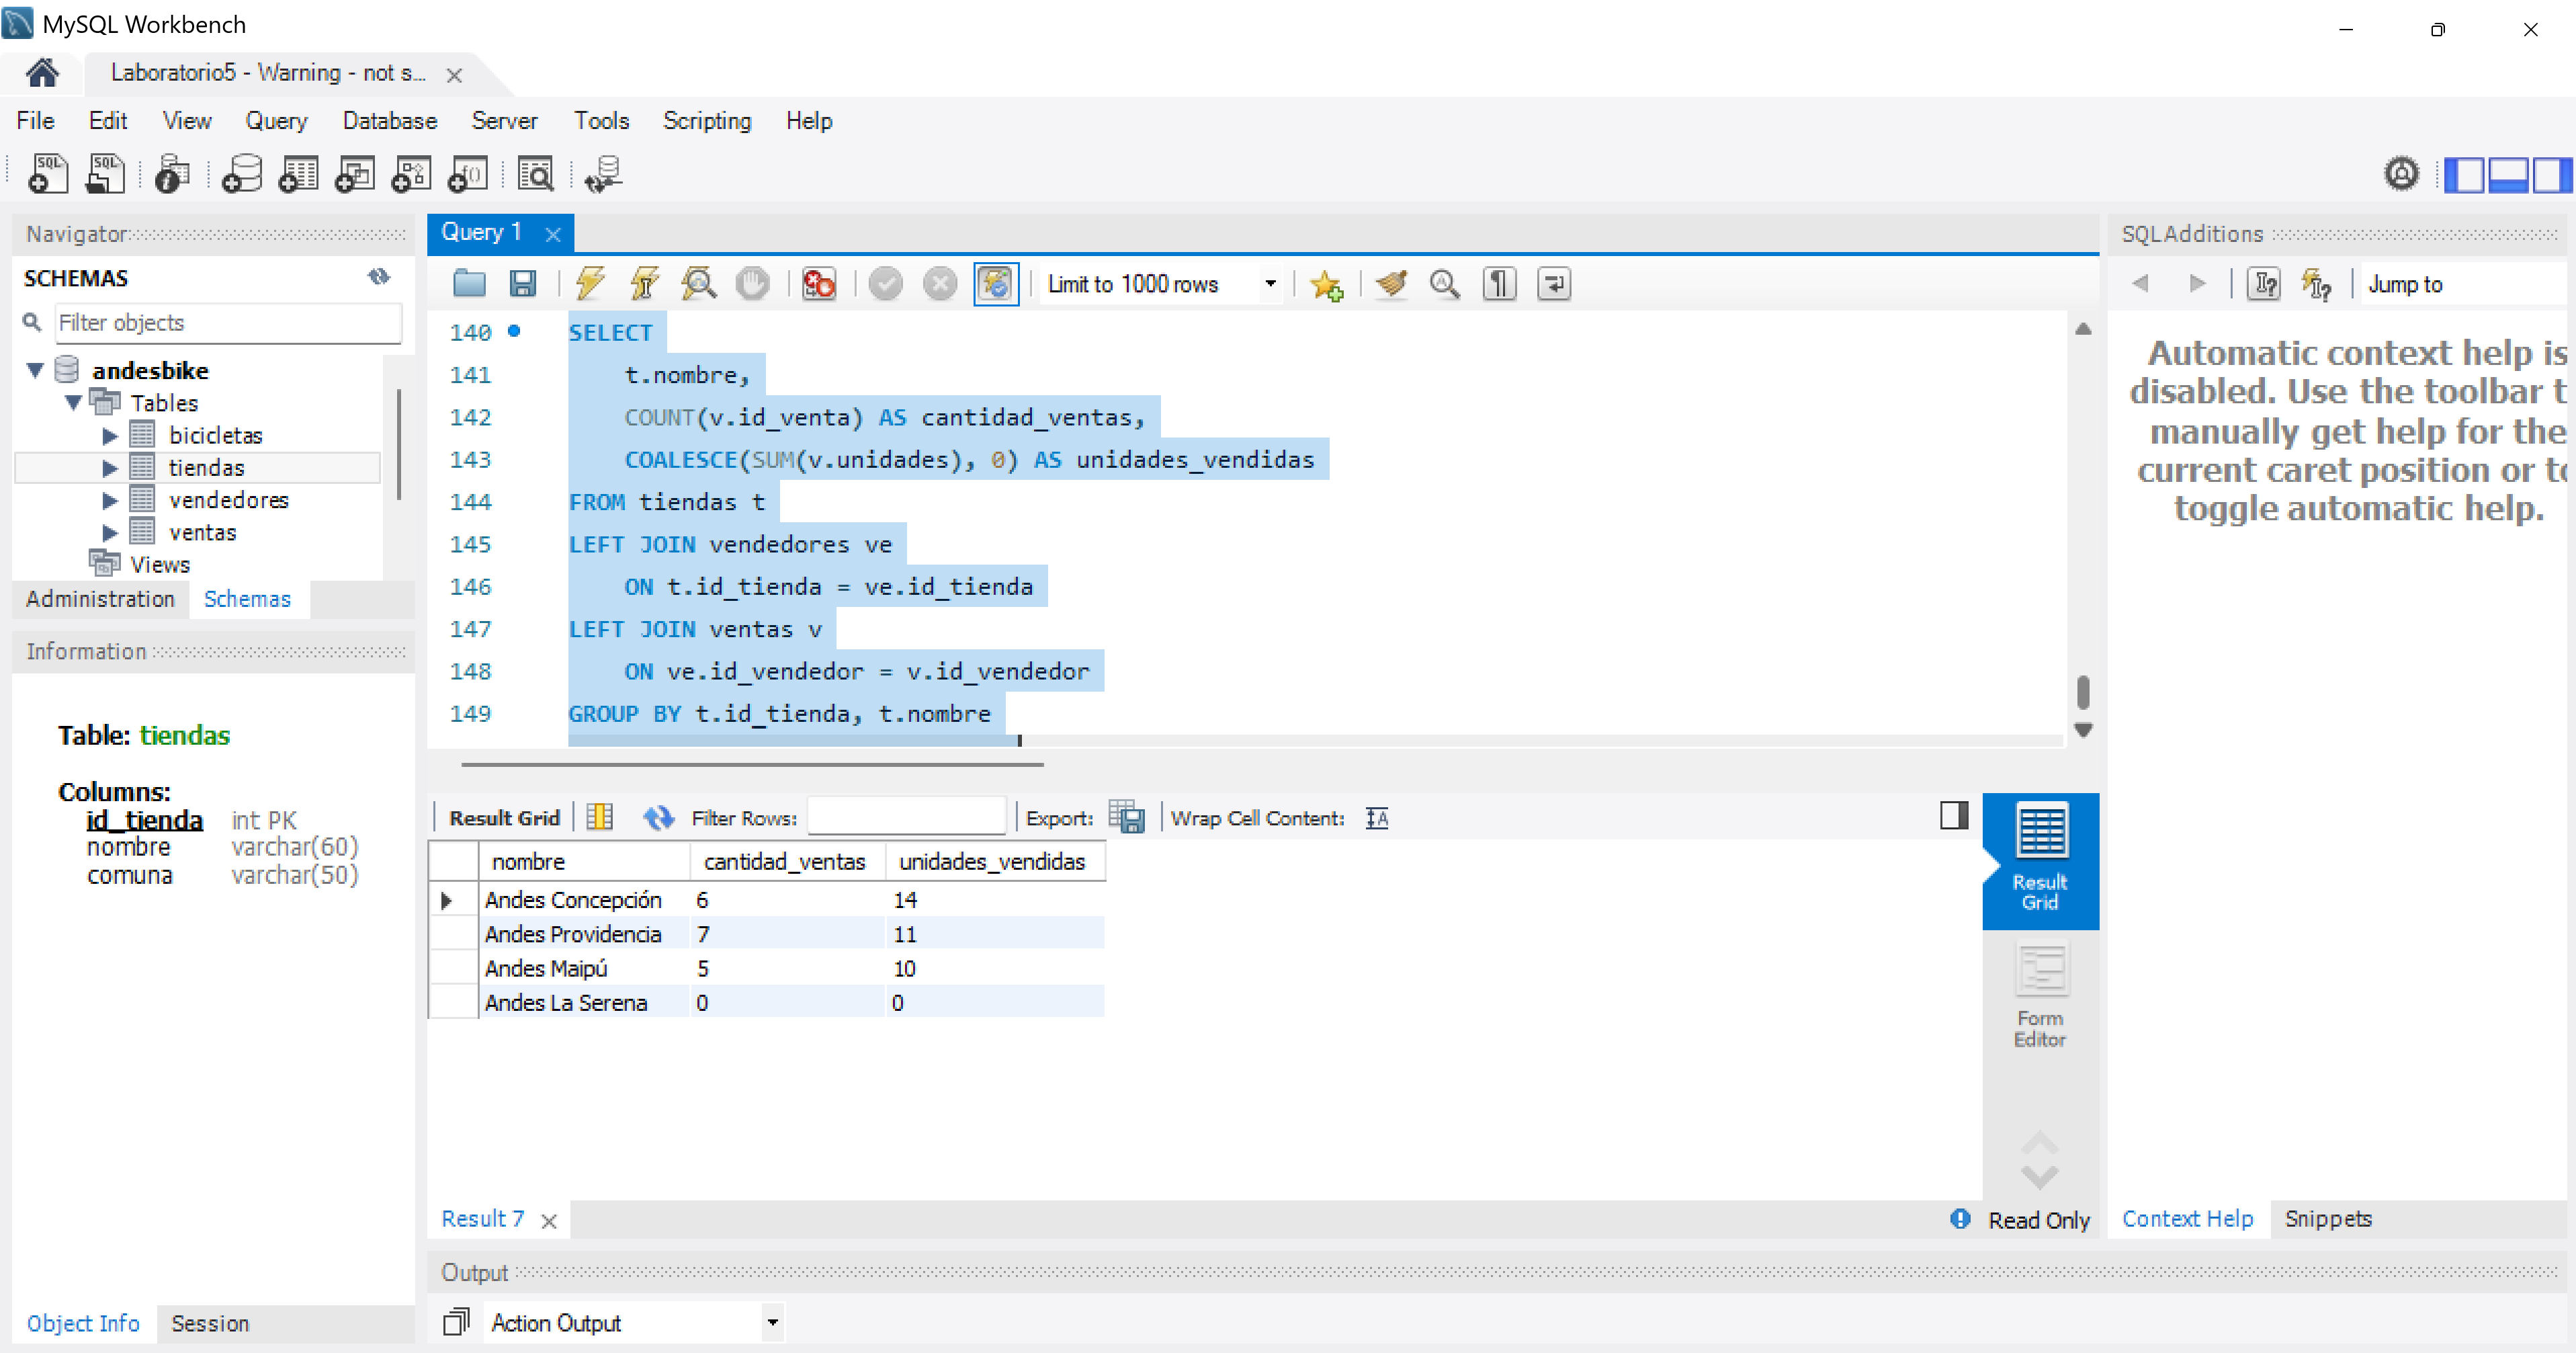
\includegraphics[width=0.95\textwidth,
height=0.38\textheight,keepaspectratio]{Consulta_02.png}
\end{figure}

\clearpage

\section*{Consulta 3}

\begin{lstlisting}[style=sqlstyle]
SELECT t.nombre
FROM tiendas t
LEFT JOIN vendedores ve
    ON t.id_tienda = ve.id_tienda
WHERE ve.id_vendedor IS NULL;
\end{lstlisting}

\begin{figure}[H]
\centering
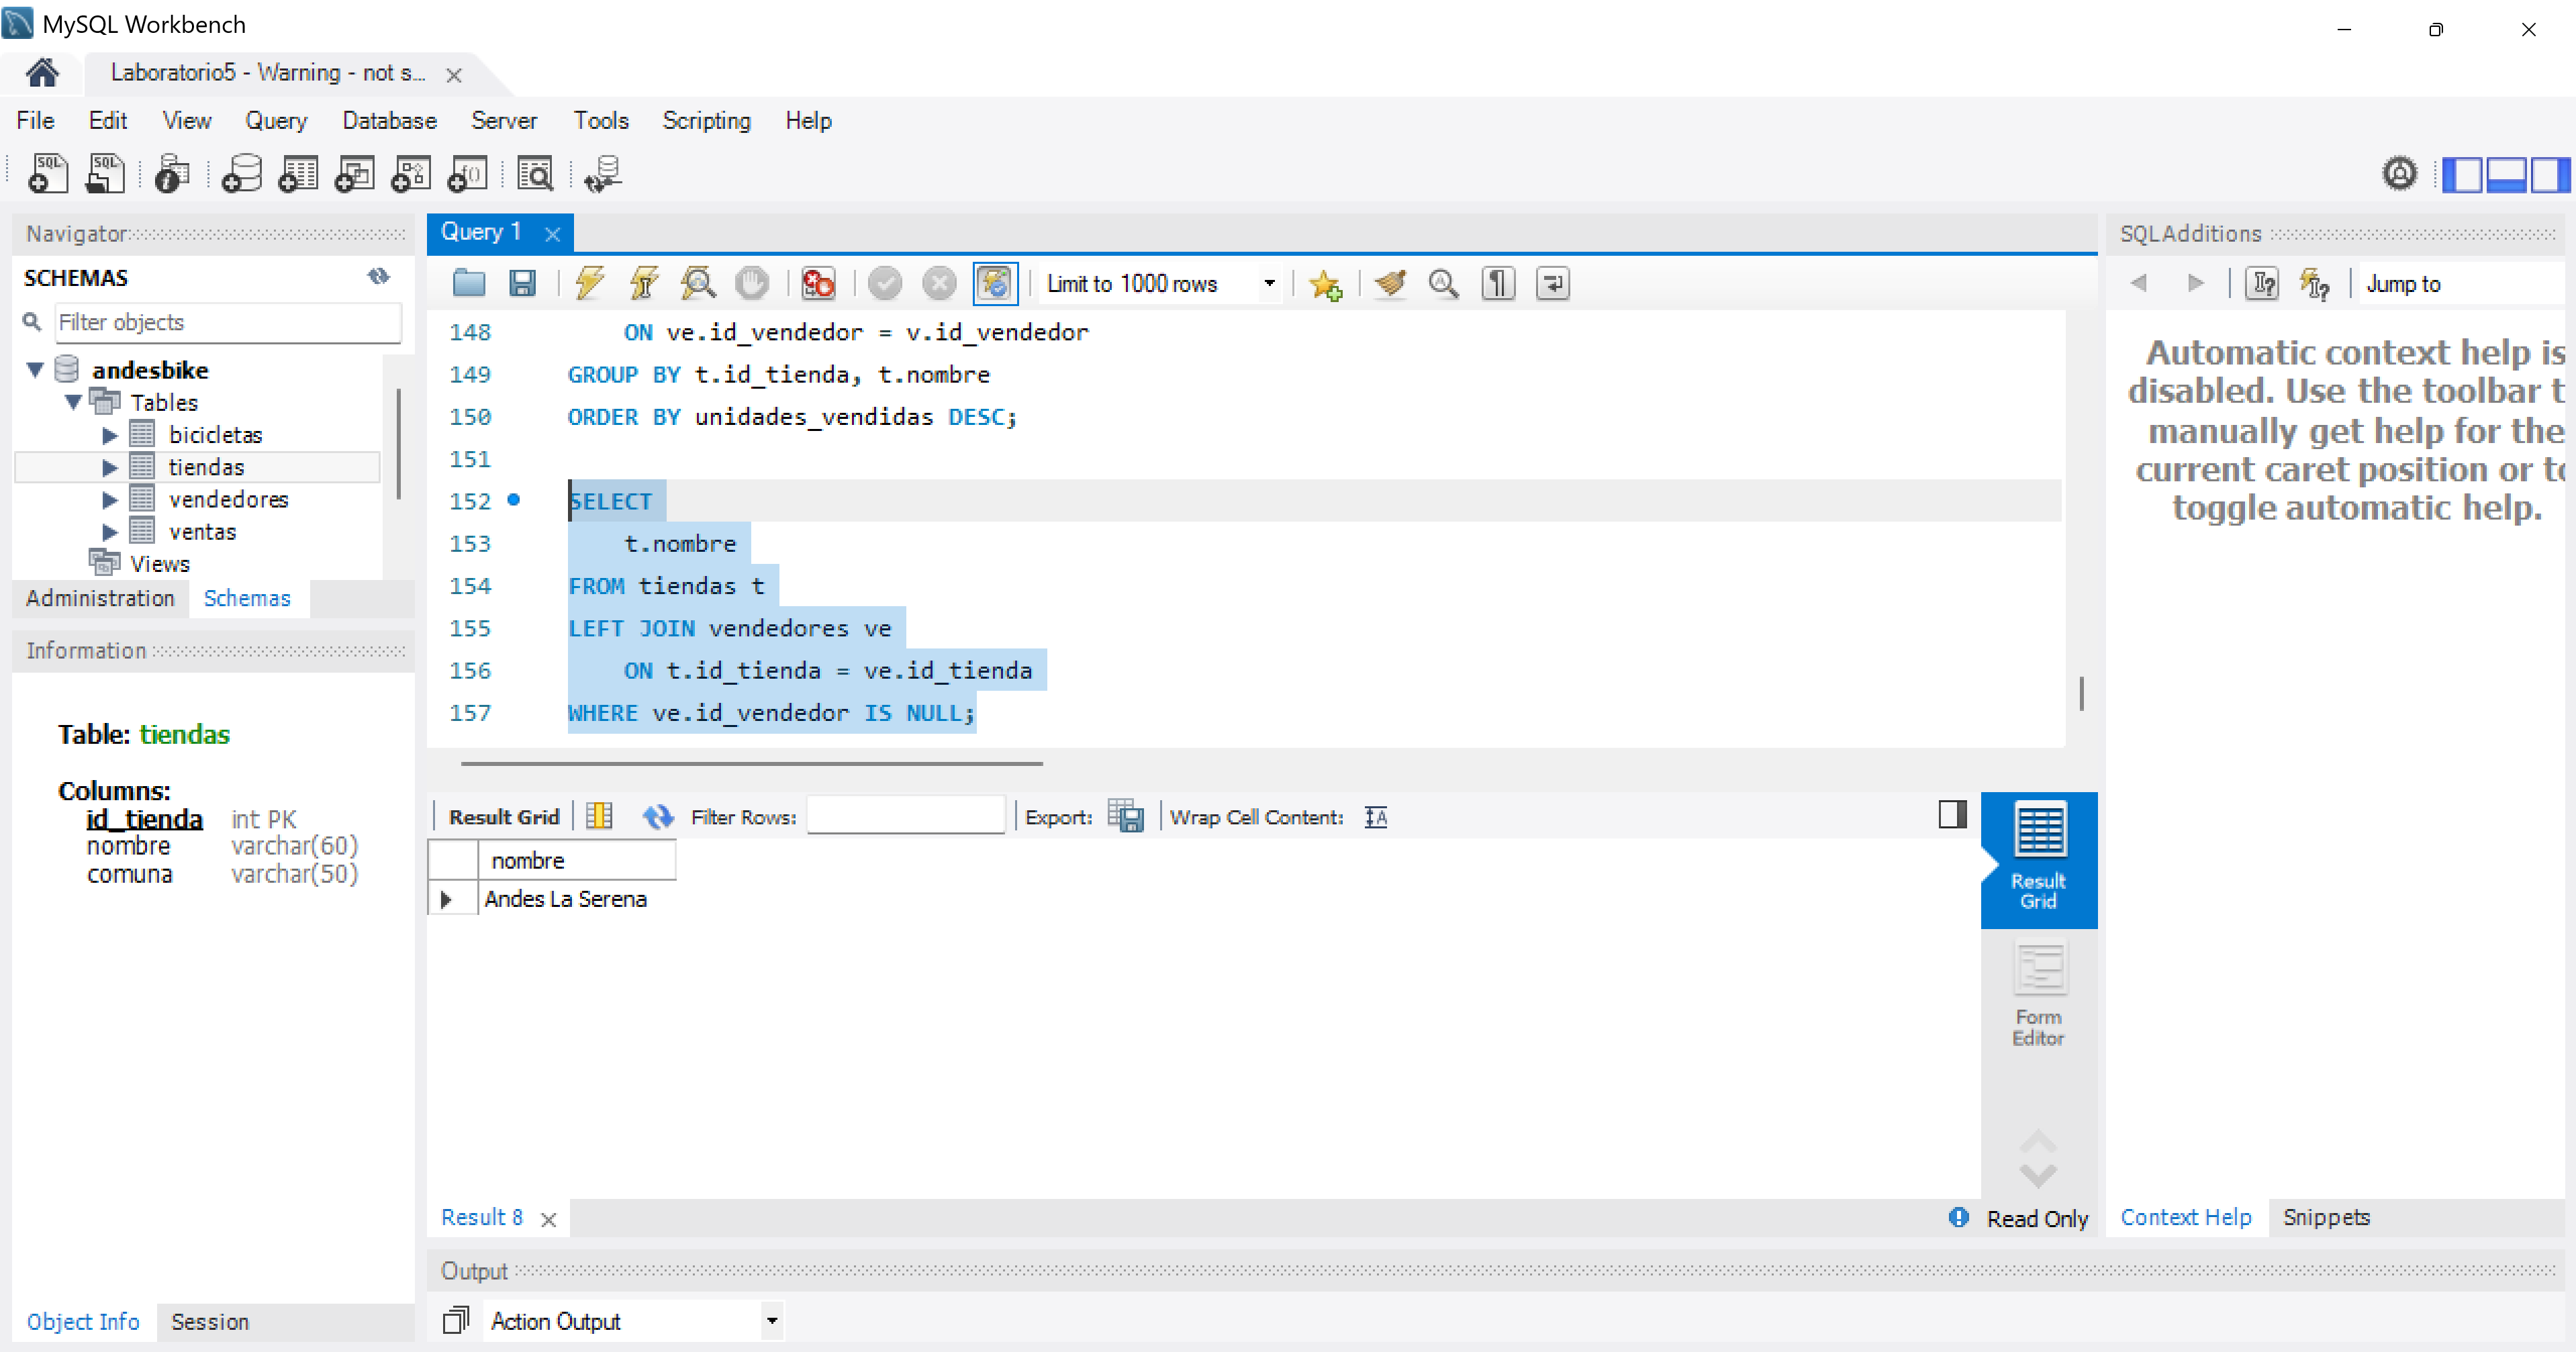
\includegraphics[width=0.95\textwidth,
height=0.38\textheight,keepaspectratio]{Consulta_03.png}
\end{figure}

\clearpage


\section*{Consulta 4}

\begin{lstlisting}[style=sqlstyle]
SELECT b.modelo
FROM bicicletas b
LEFT JOIN ventas v
    ON b.id_bicicleta = v.id_bicicleta
    AND v.fecha >= '2025-06-01'
    AND v.fecha < '2025-07-01'
WHERE v.id_venta IS NULL
ORDER BY b.modelo;
\end{lstlisting}

\noindent
La condición de fecha se coloca en el
\texttt{ON} para considerar únicamente las ventas de junio
y conservar todas las bicicletas, permitiendo identificar
aquellas que no tuvieron ventas durante ese período.

\begin{figure}[H]
\centering
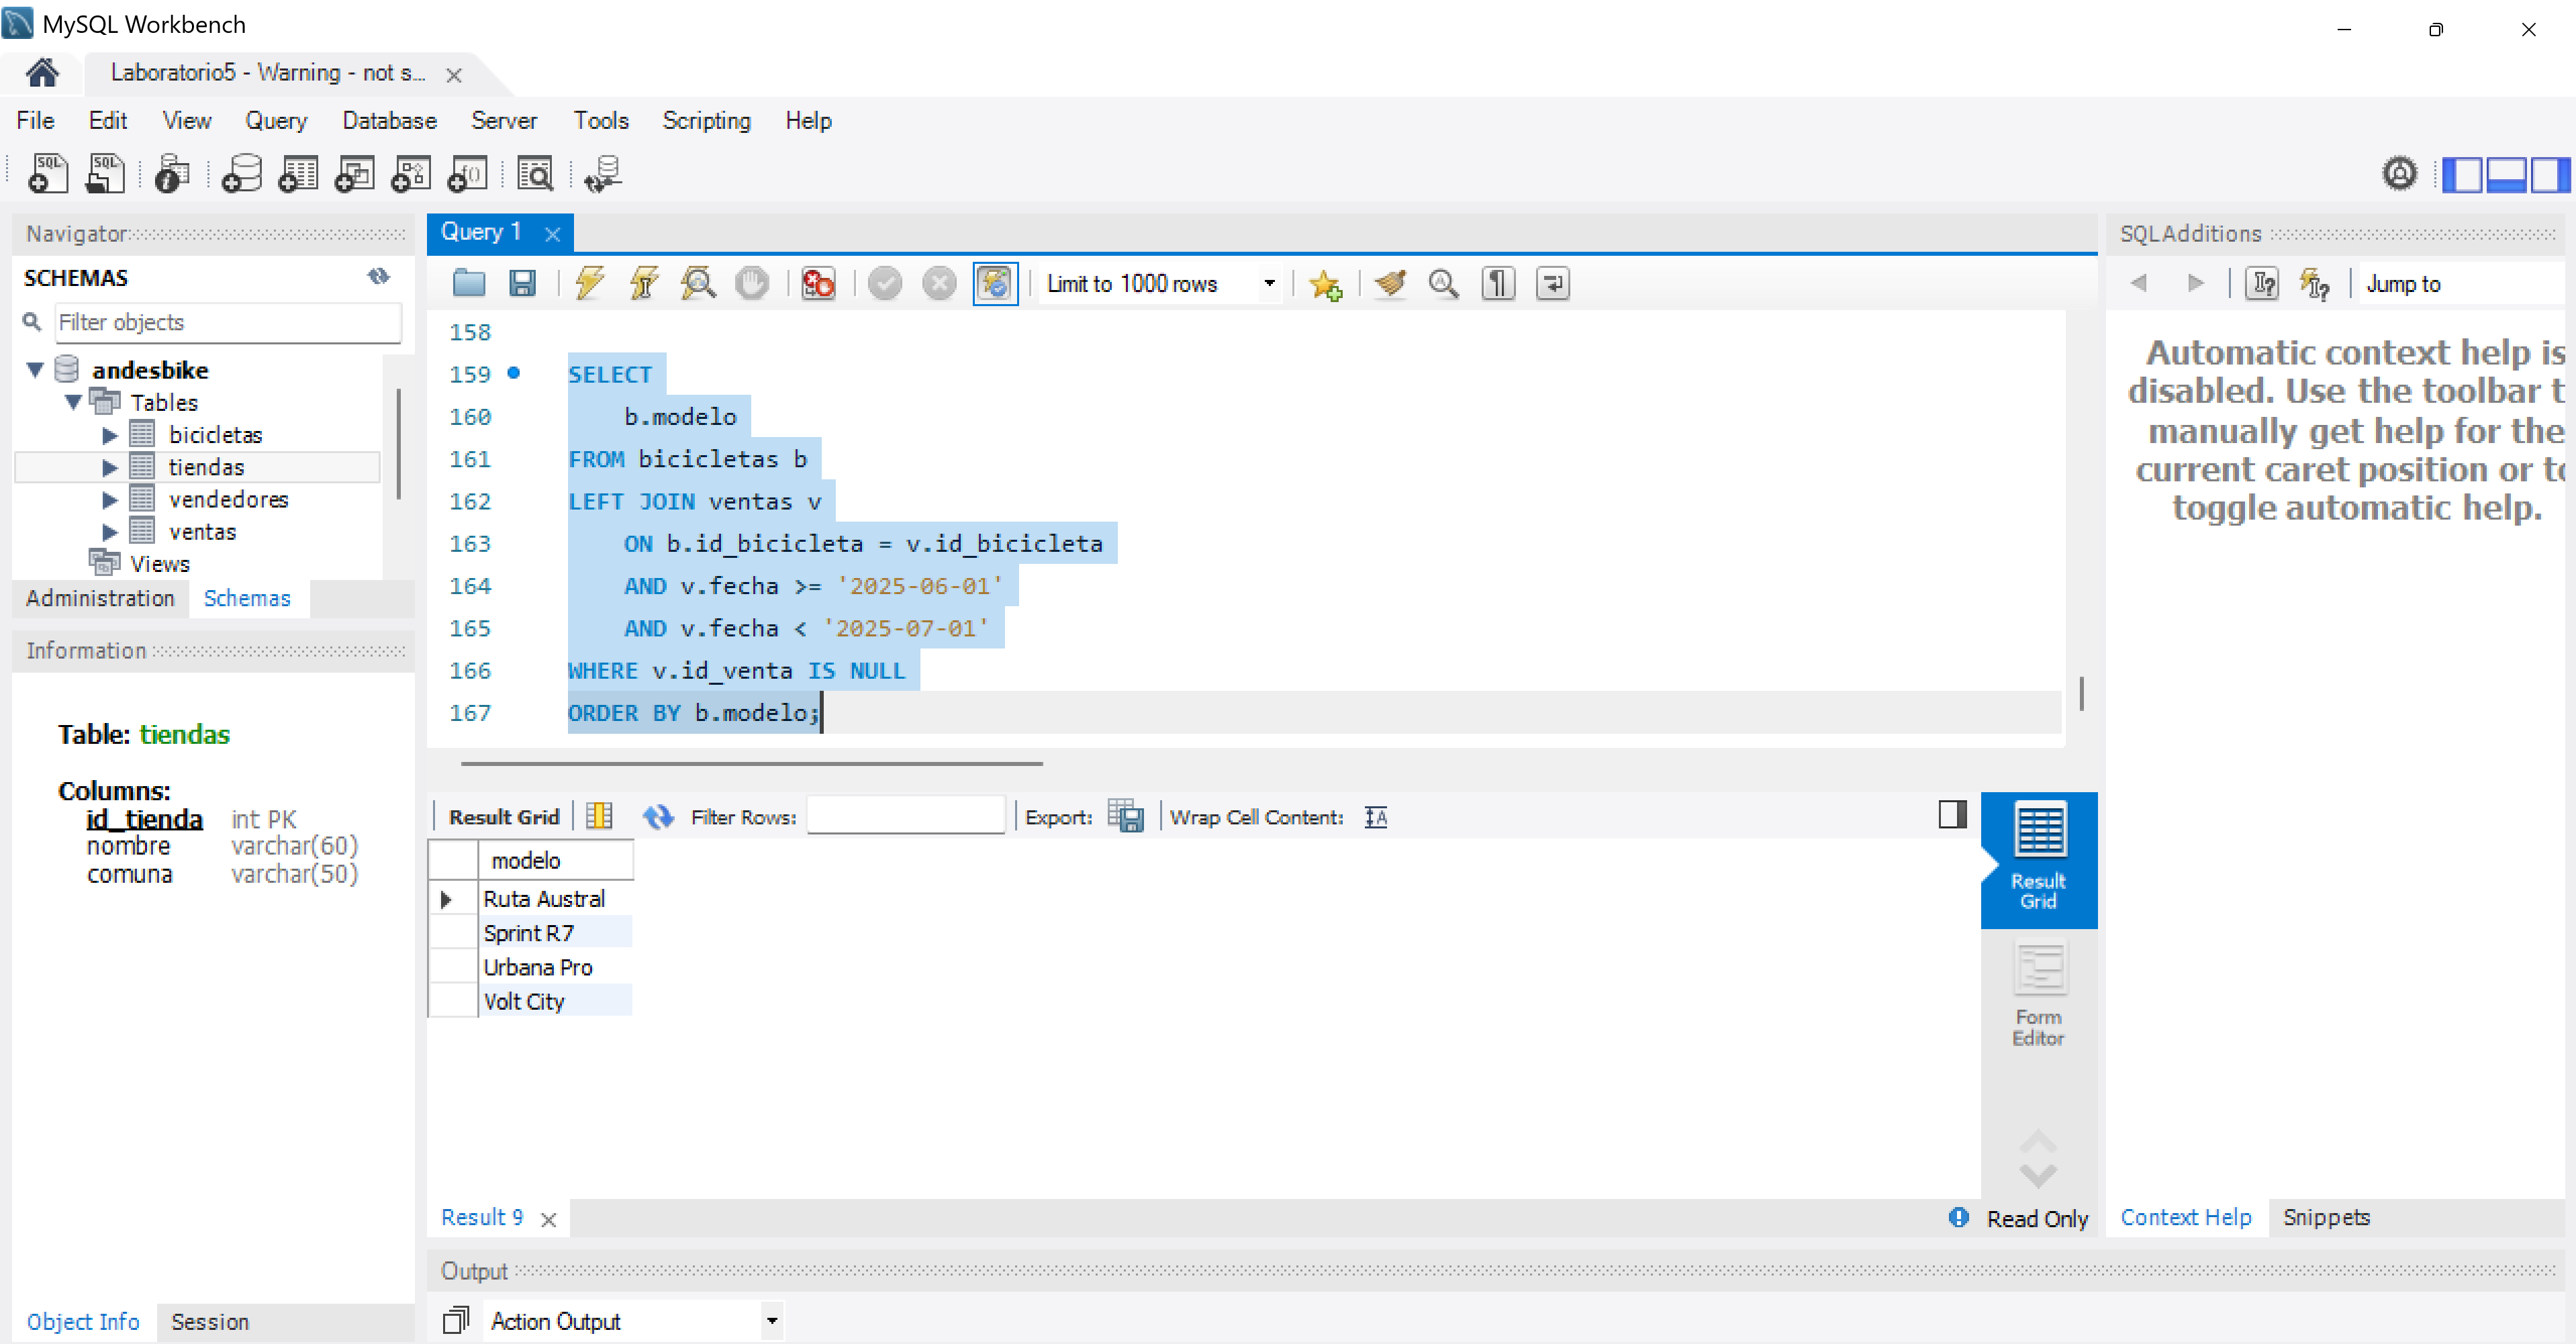
\includegraphics[width=0.95\textwidth,
height=0.38\textheight,keepaspectratio]{Consulta_04.png}
\end{figure}

\clearpage


\section*{Consulta 5}

\begin{lstlisting}[style=sqlstyle]
SELECT ve.nombre AS vendedor,
       COALESCE(t.nombre, 'Sin tienda asignada') AS tienda
FROM vendedores ve
LEFT JOIN tiendas t
    ON ve.id_tienda = t.id_tienda
LEFT JOIN ventas v
    ON ve.id_vendedor = v.id_vendedor
WHERE v.id_venta IS NULL
ORDER BY ve.nombre ASC;
\end{lstlisting}

\begin{figure}[H]
\centering
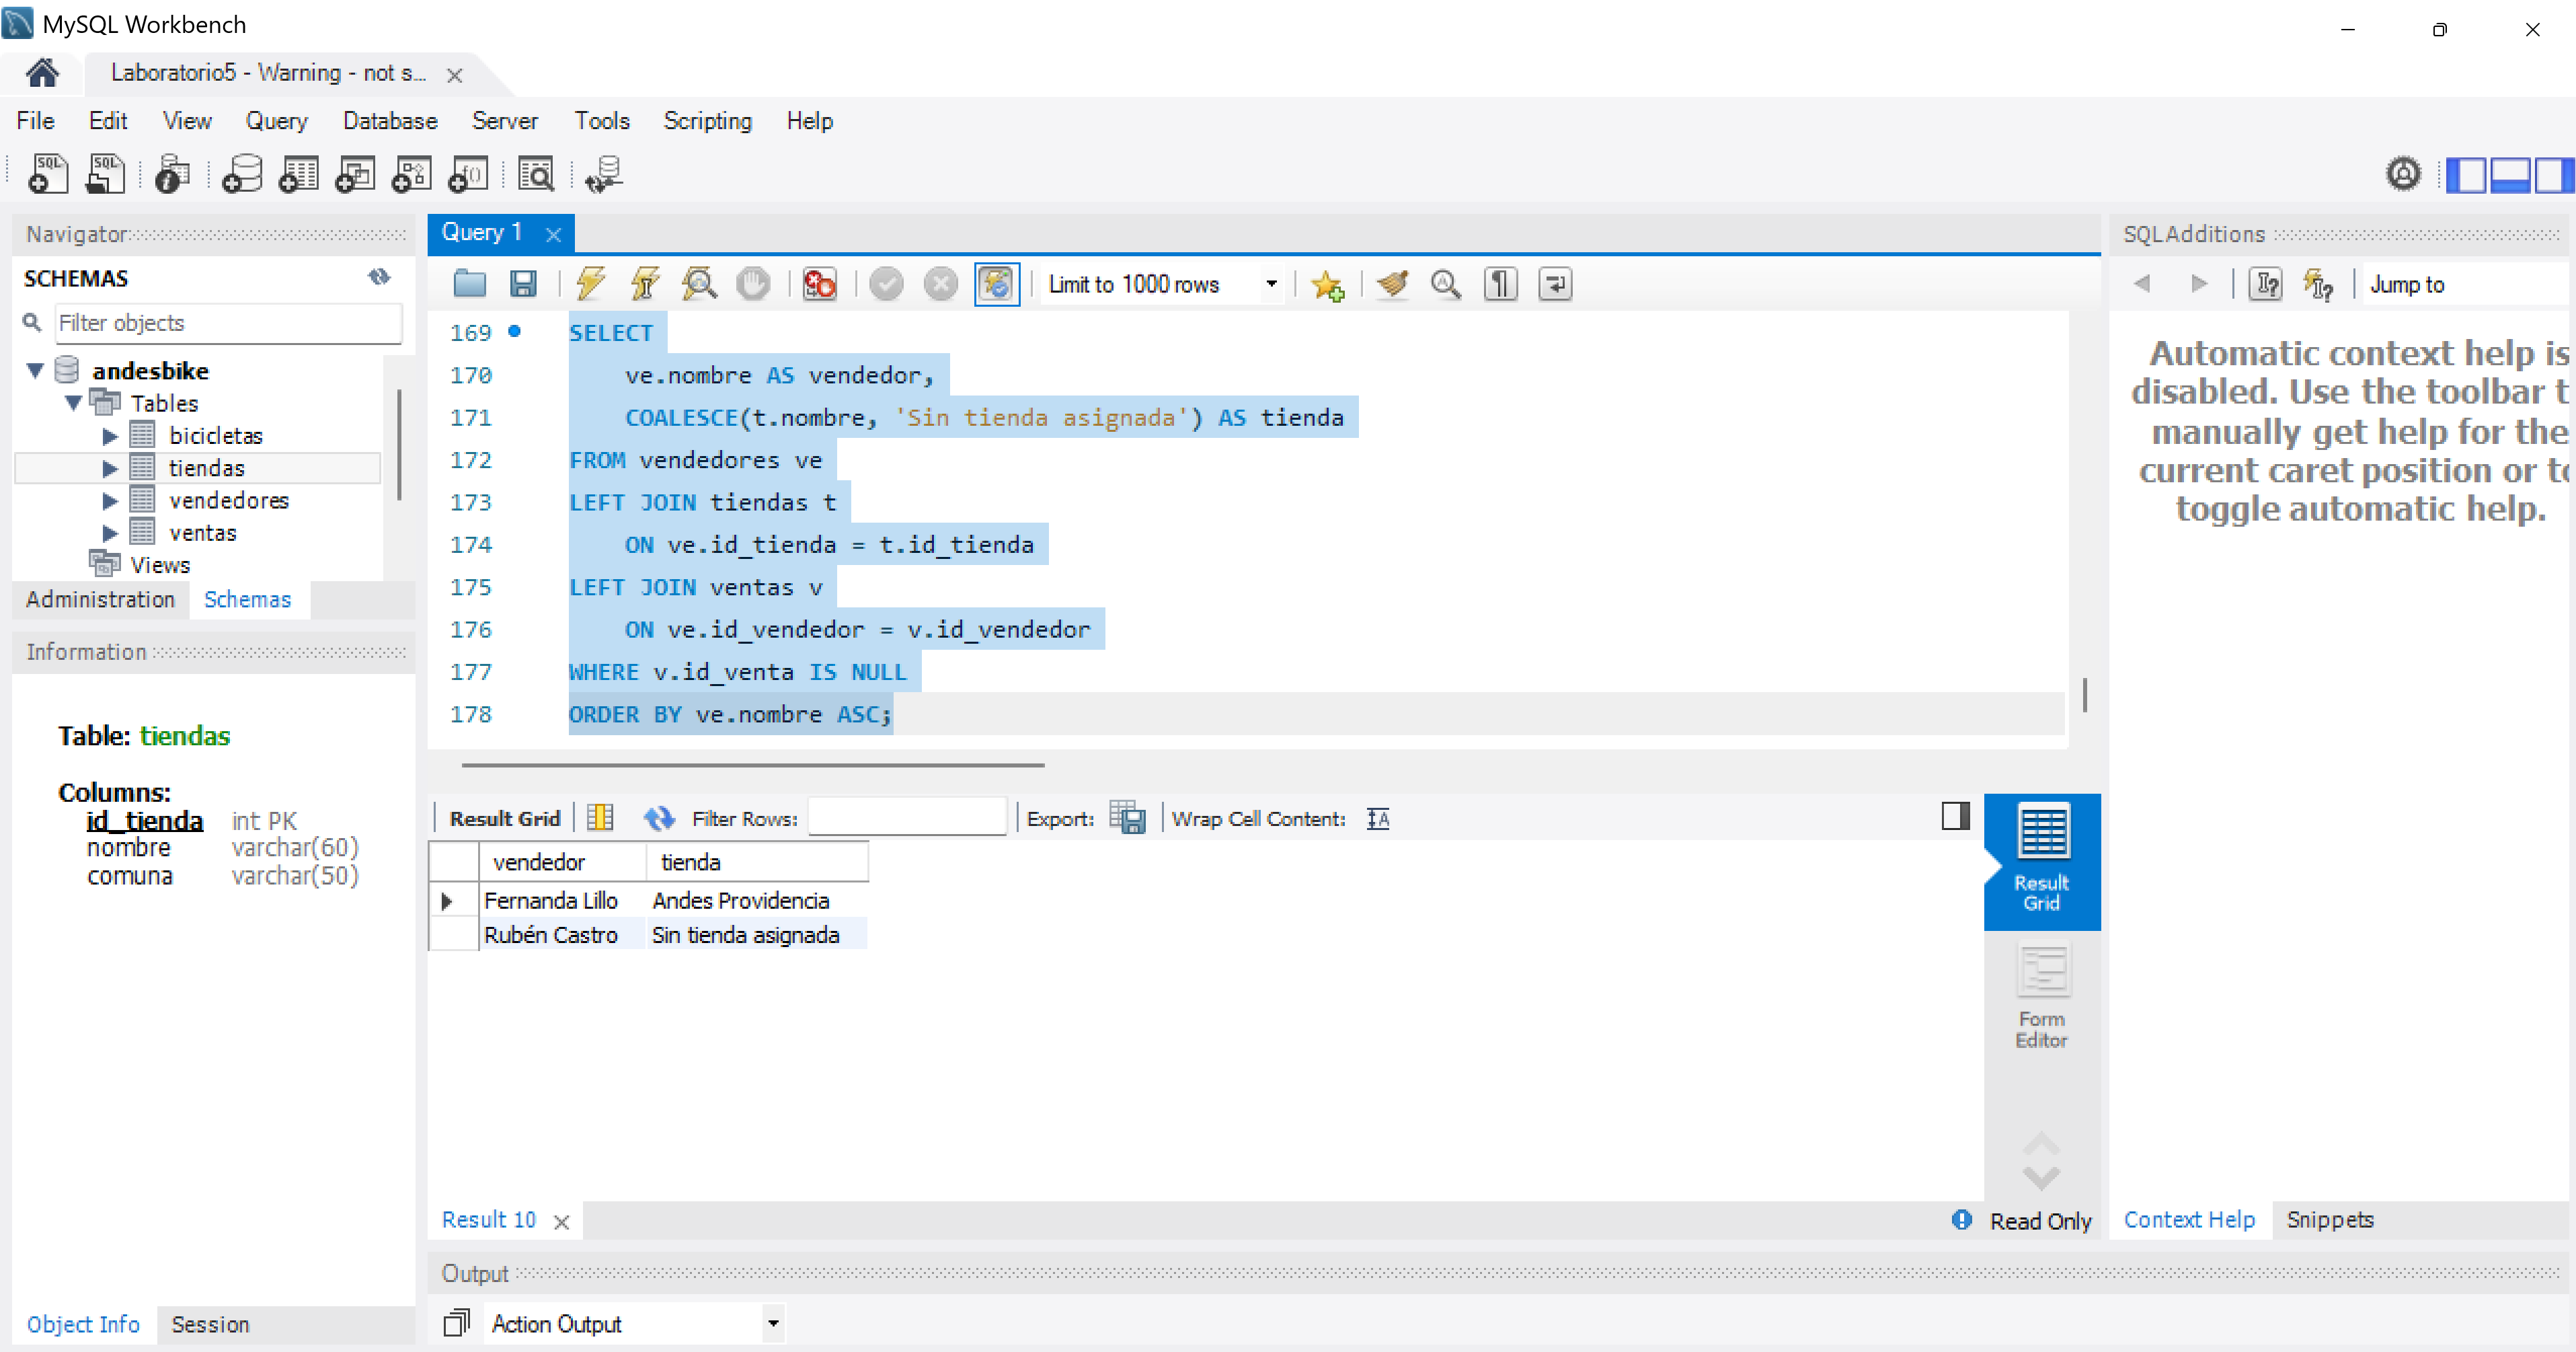
\includegraphics[width=0.95\textwidth,
height=0.38\textheight,keepaspectratio]{Consulta_05.png}
\end{figure}

\clearpage


\section*{Consulta 6}

\begin{lstlisting}[style=sqlstyle]
SELECT v1.nombre AS vendedor_1,
       v1.fecha_ingreso AS fecha_ingreso_1,
       v2.nombre AS vendedor_2,
       v2.fecha_ingreso AS fecha_ingreso_2,
       t.nombre AS tienda
FROM vendedores v1
JOIN vendedores v2
    ON v1.id_tienda = v2.id_tienda
    AND v1.fecha_ingreso < v2.fecha_ingreso
JOIN tiendas t
    ON v1.id_tienda = t.id_tienda
ORDER BY t.nombre, v1.fecha_ingreso;
\end{lstlisting}

\begin{figure}[H]
\centering
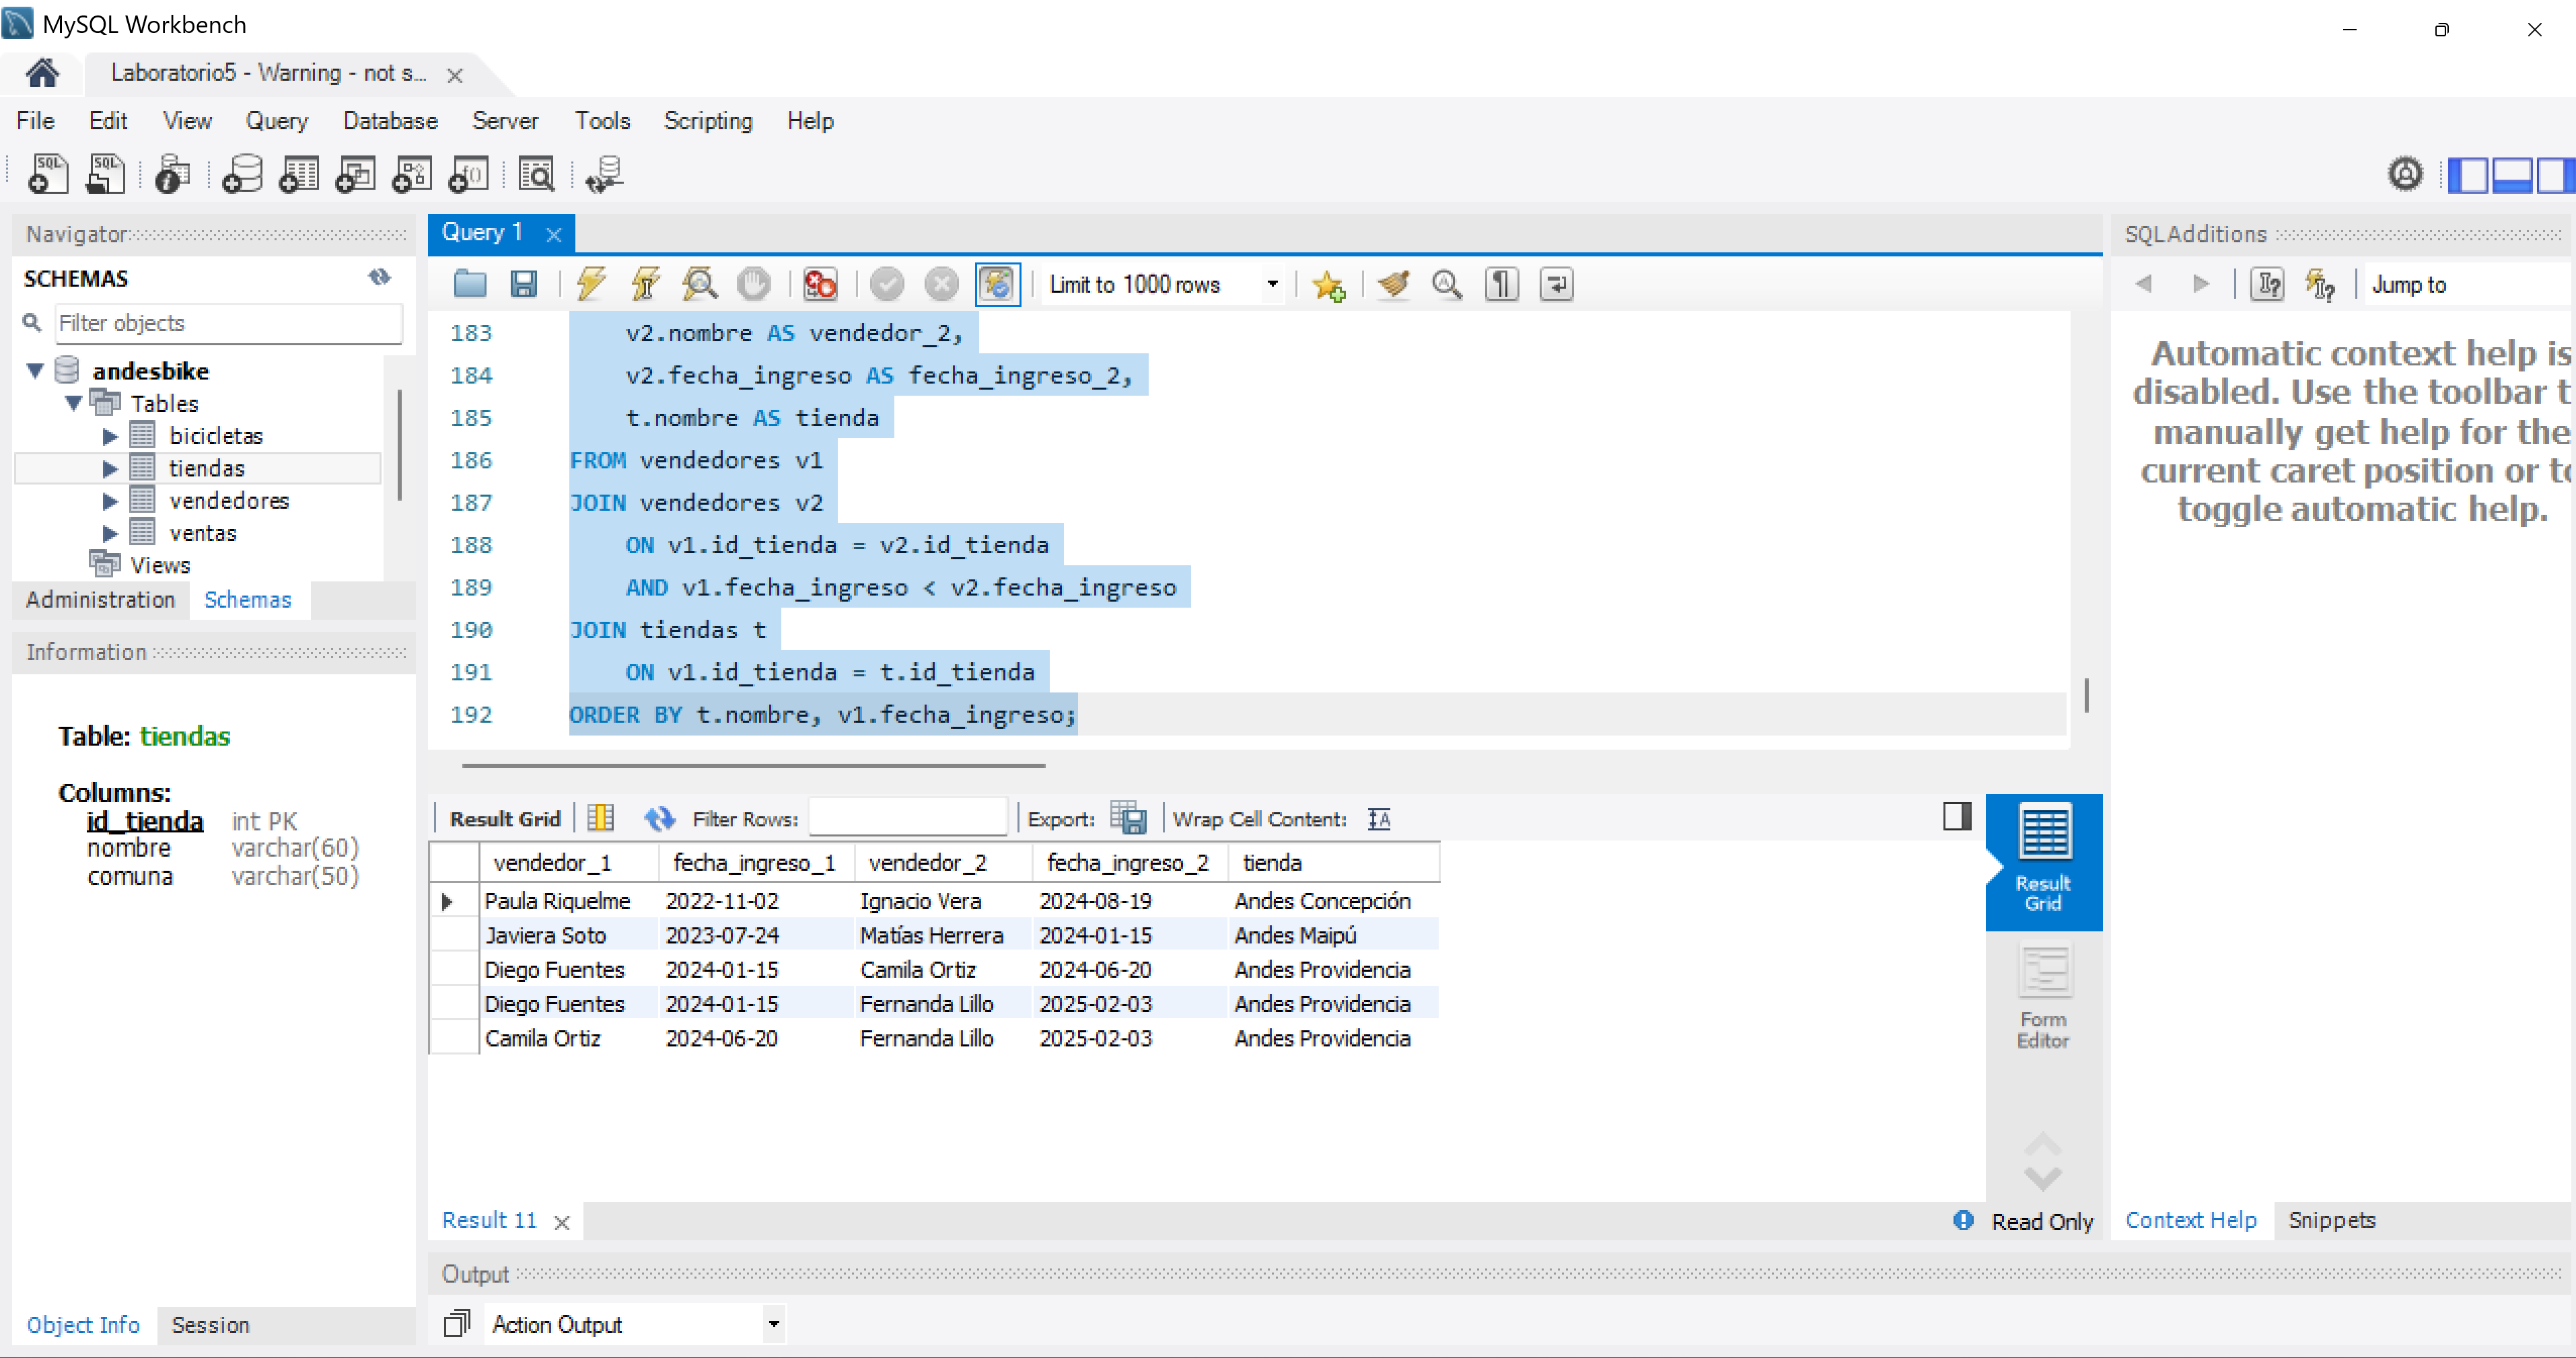
\includegraphics[width=0.95\textwidth,
height=0.38\textheight,keepaspectratio]{Consulta_06.png}
\end{figure}

\clearpage


\section*{Consulta 7}

\begin{lstlisting}[style=sqlstyle]
SELECT t.nombre AS tienda,
       SUM(v.unidades * b.precio) AS monto_total
FROM tiendas t
JOIN vendedores ve
    ON t.id_tienda = ve.id_tienda
JOIN ventas v
    ON ve.id_vendedor = v.id_vendedor
JOIN bicicletas b
    ON v.id_bicicleta = b.id_bicicleta
WHERE b.categoria IN ('Montania', 'Ruta')
GROUP BY t.id_tienda, t.nombre
HAVING SUM(v.unidades * b.precio) > 2000000
ORDER BY monto_total DESC;
\end{lstlisting}

\begin{figure}[H]
\centering
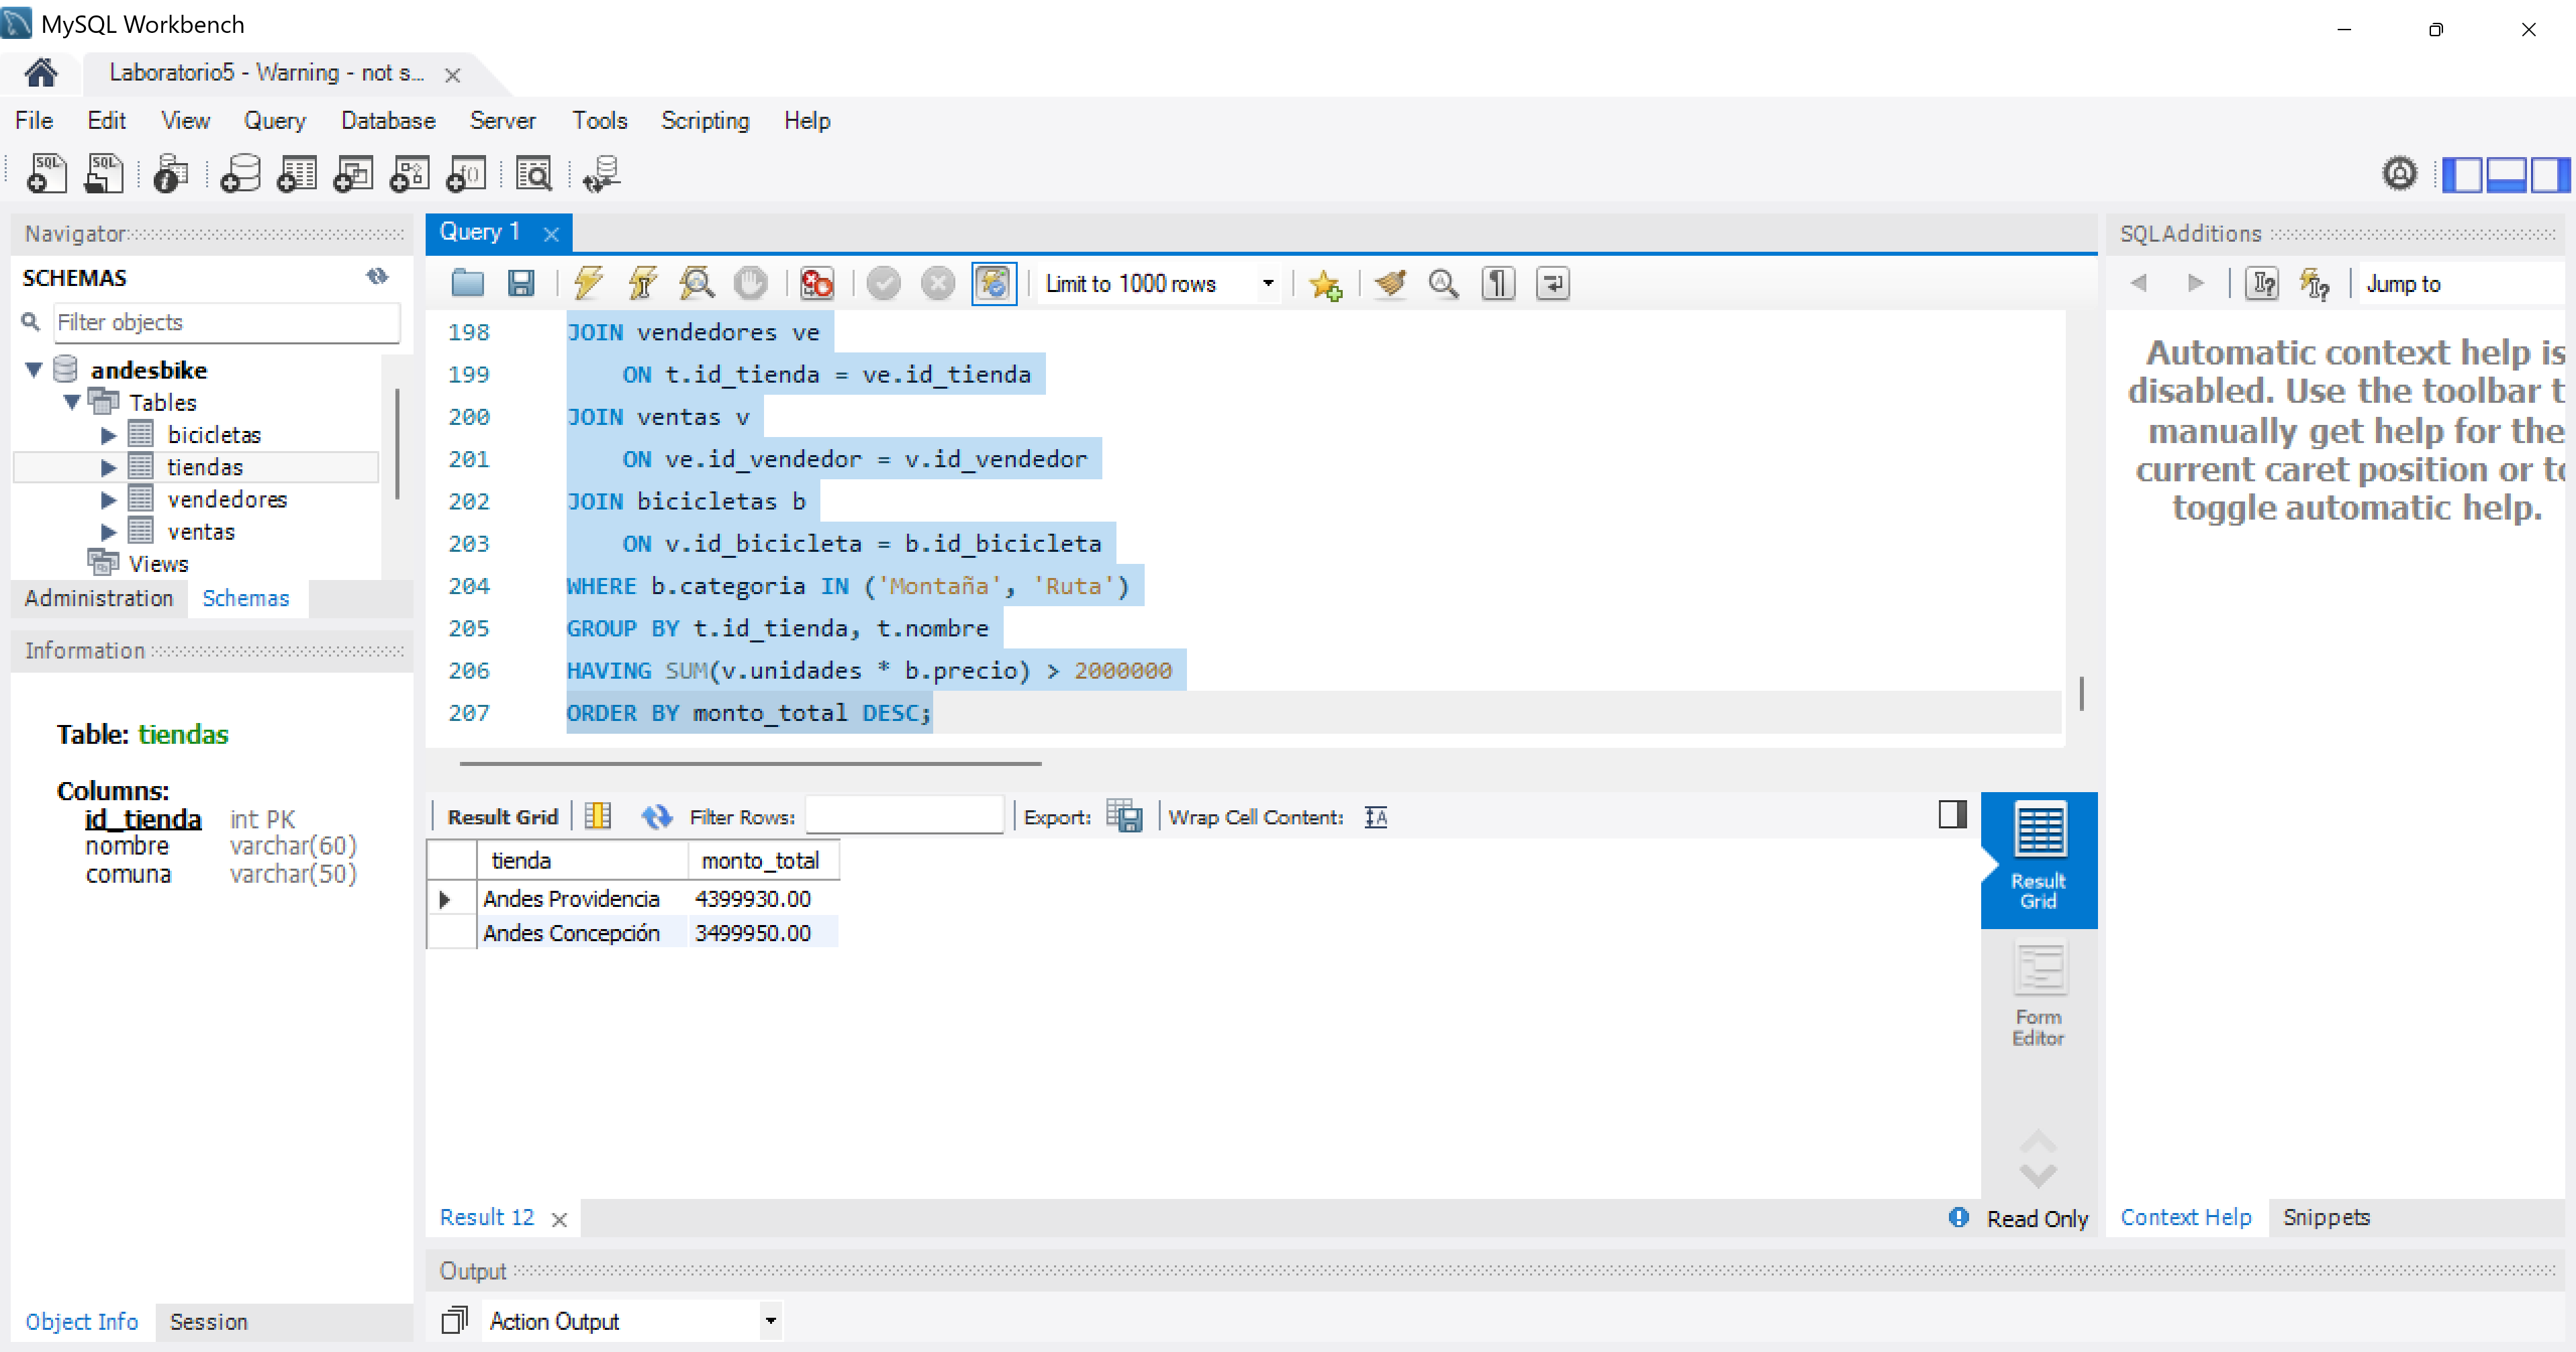
\includegraphics[width=0.95\textwidth,
height=0.38\textheight,keepaspectratio]{Consulta_07.png}
\end{figure}

\clearpage


\section*{Consulta 8}

\begin{lstlisting}[style=sqlstyle]
SELECT modelo,
       precio
FROM bicicletas
WHERE precio > (
    SELECT AVG(precio)
    FROM bicicletas
)
ORDER BY precio DESC;
\end{lstlisting}

\noindent
 La subconsulta calcula el precio
promedio de todo el catálogo, cuyo valor es \$657.490,
utilizando la función \texttt{AVG(precio)} sobre los
registros de la tabla bicicletas. Posteriormente,
se muestran los modelos cuyo precio supera dicho promedio.

\begin{figure}[H]
\centering
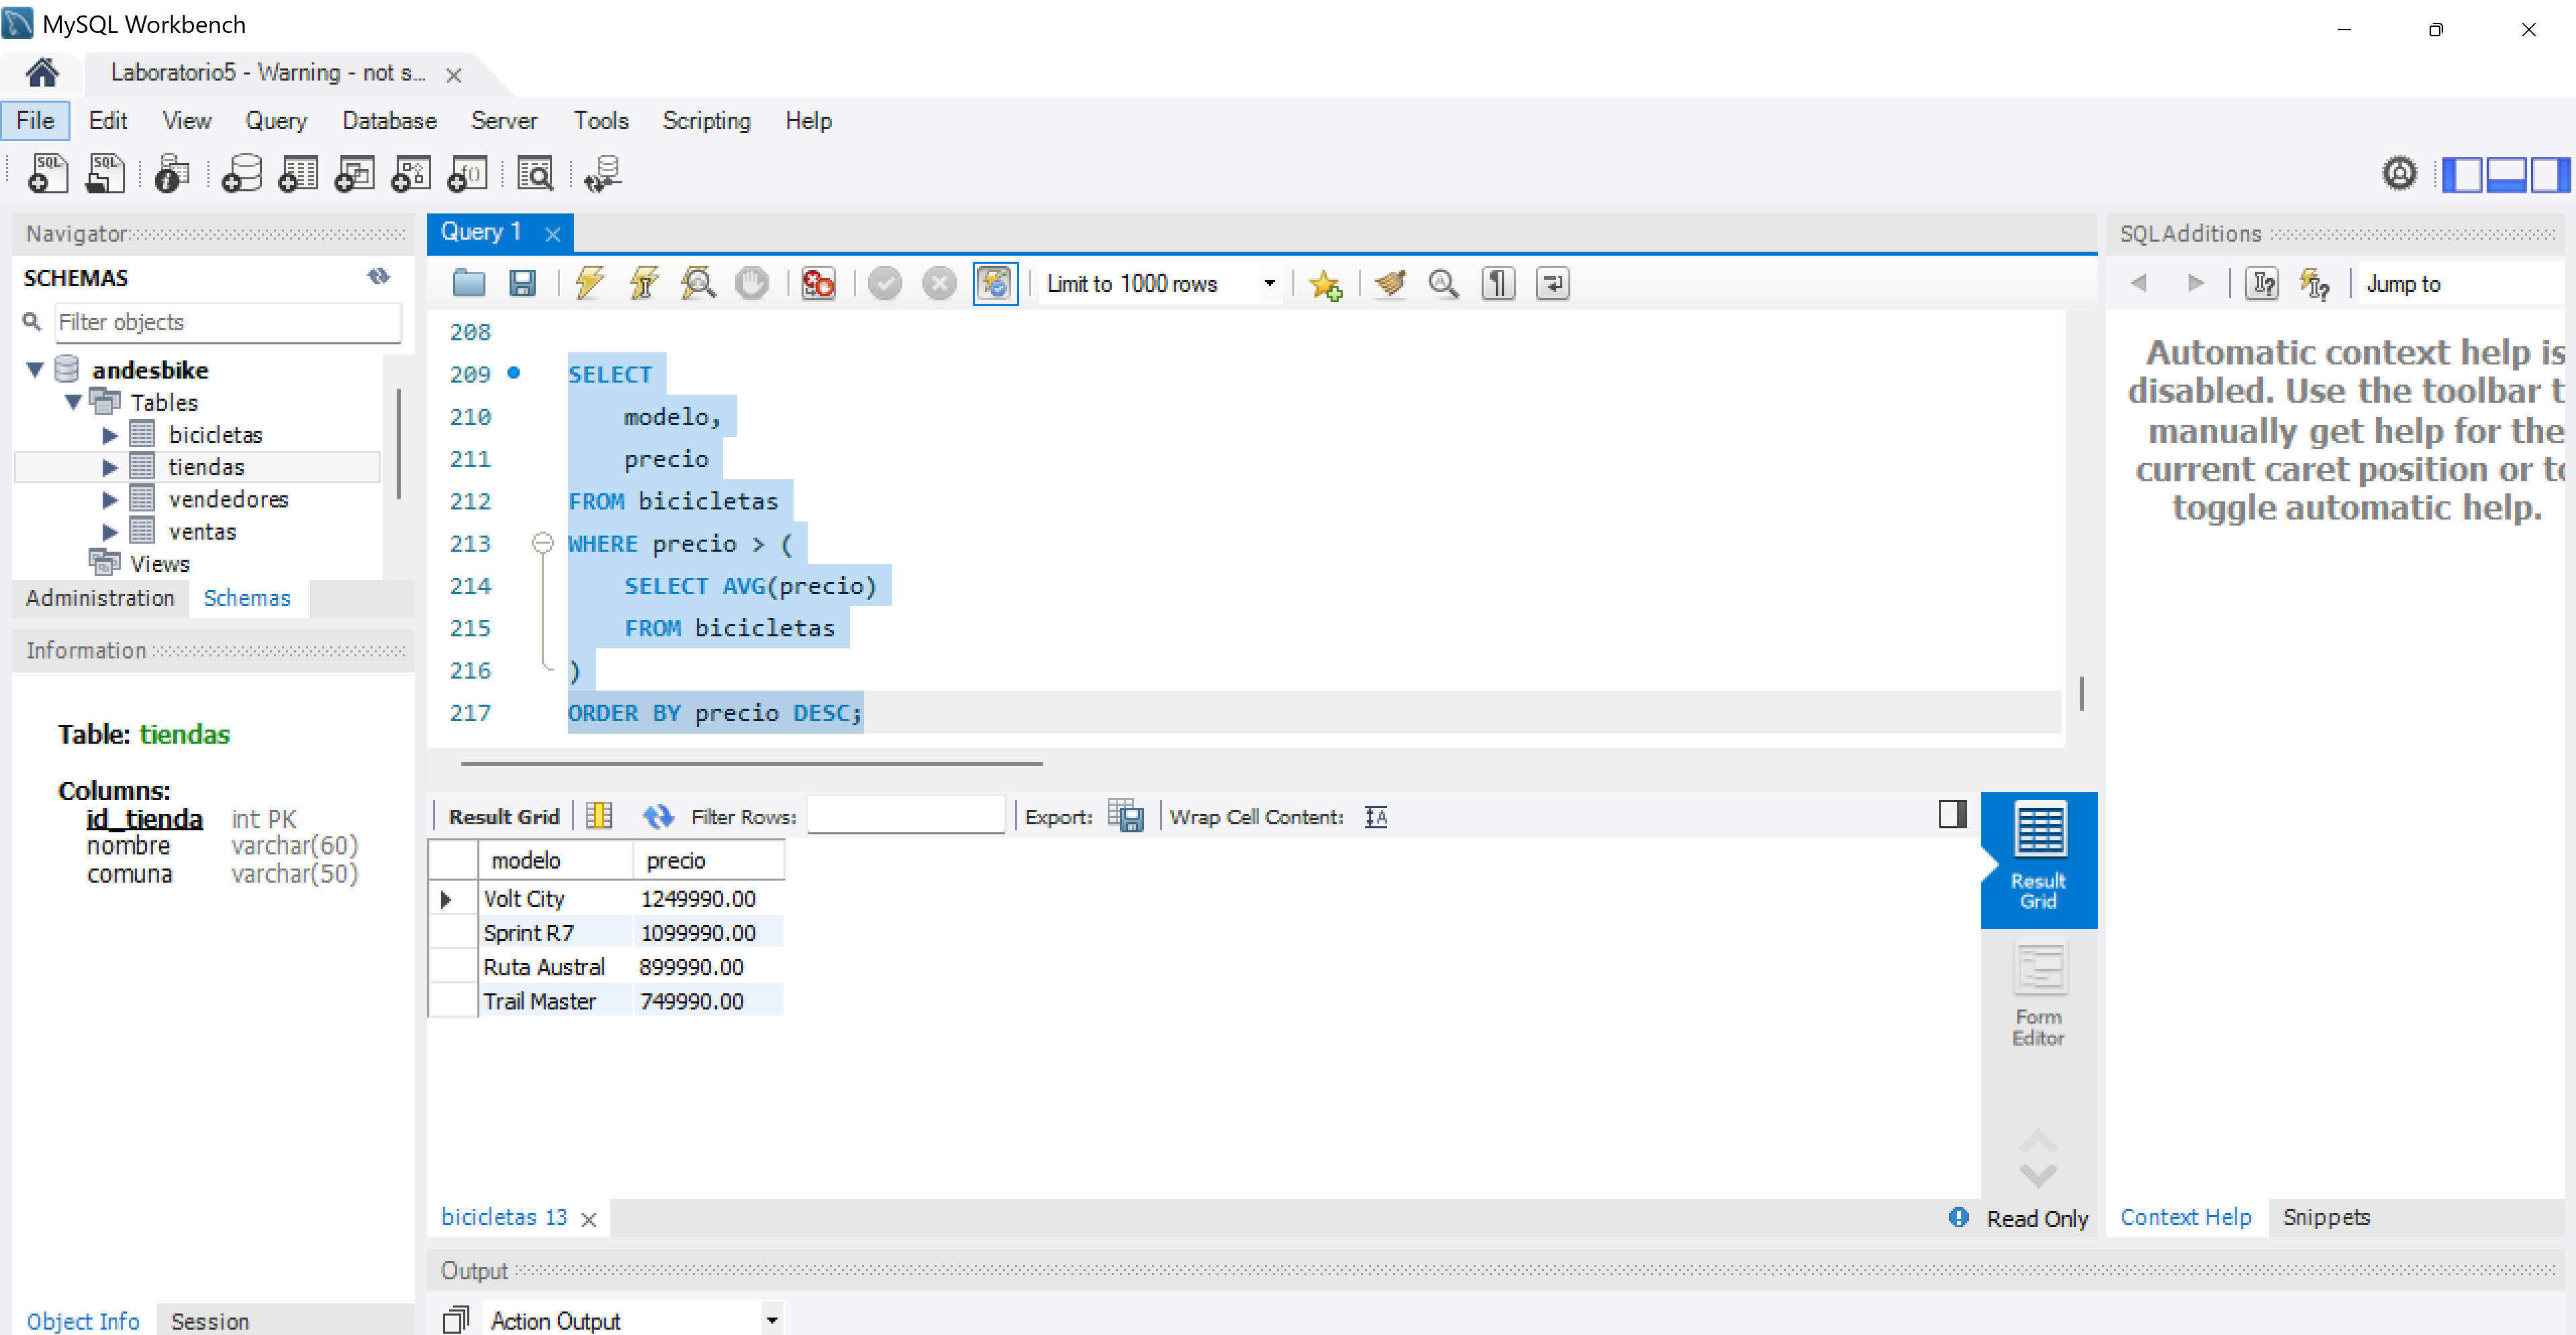
\includegraphics[width=0.95\textwidth,
height=0.38\textheight,keepaspectratio]{Consulta_08.png}
\end{figure}

\clearpage


\section*{Consulta 9}

\begin{lstlisting}[style=sqlstyle]
SELECT ve.nombre,
       AVG(v.unidades) AS promedio_unidades
FROM vendedores ve
JOIN ventas v
    ON ve.id_vendedor = v.id_vendedor
GROUP BY ve.id_vendedor, ve.nombre
HAVING AVG(v.unidades) > (
    SELECT AVG(unidades)
    FROM ventas
)
ORDER BY promedio_unidades DESC, ve.nombre ASC;
\end{lstlisting}

\begin{figure}[H]
\centering
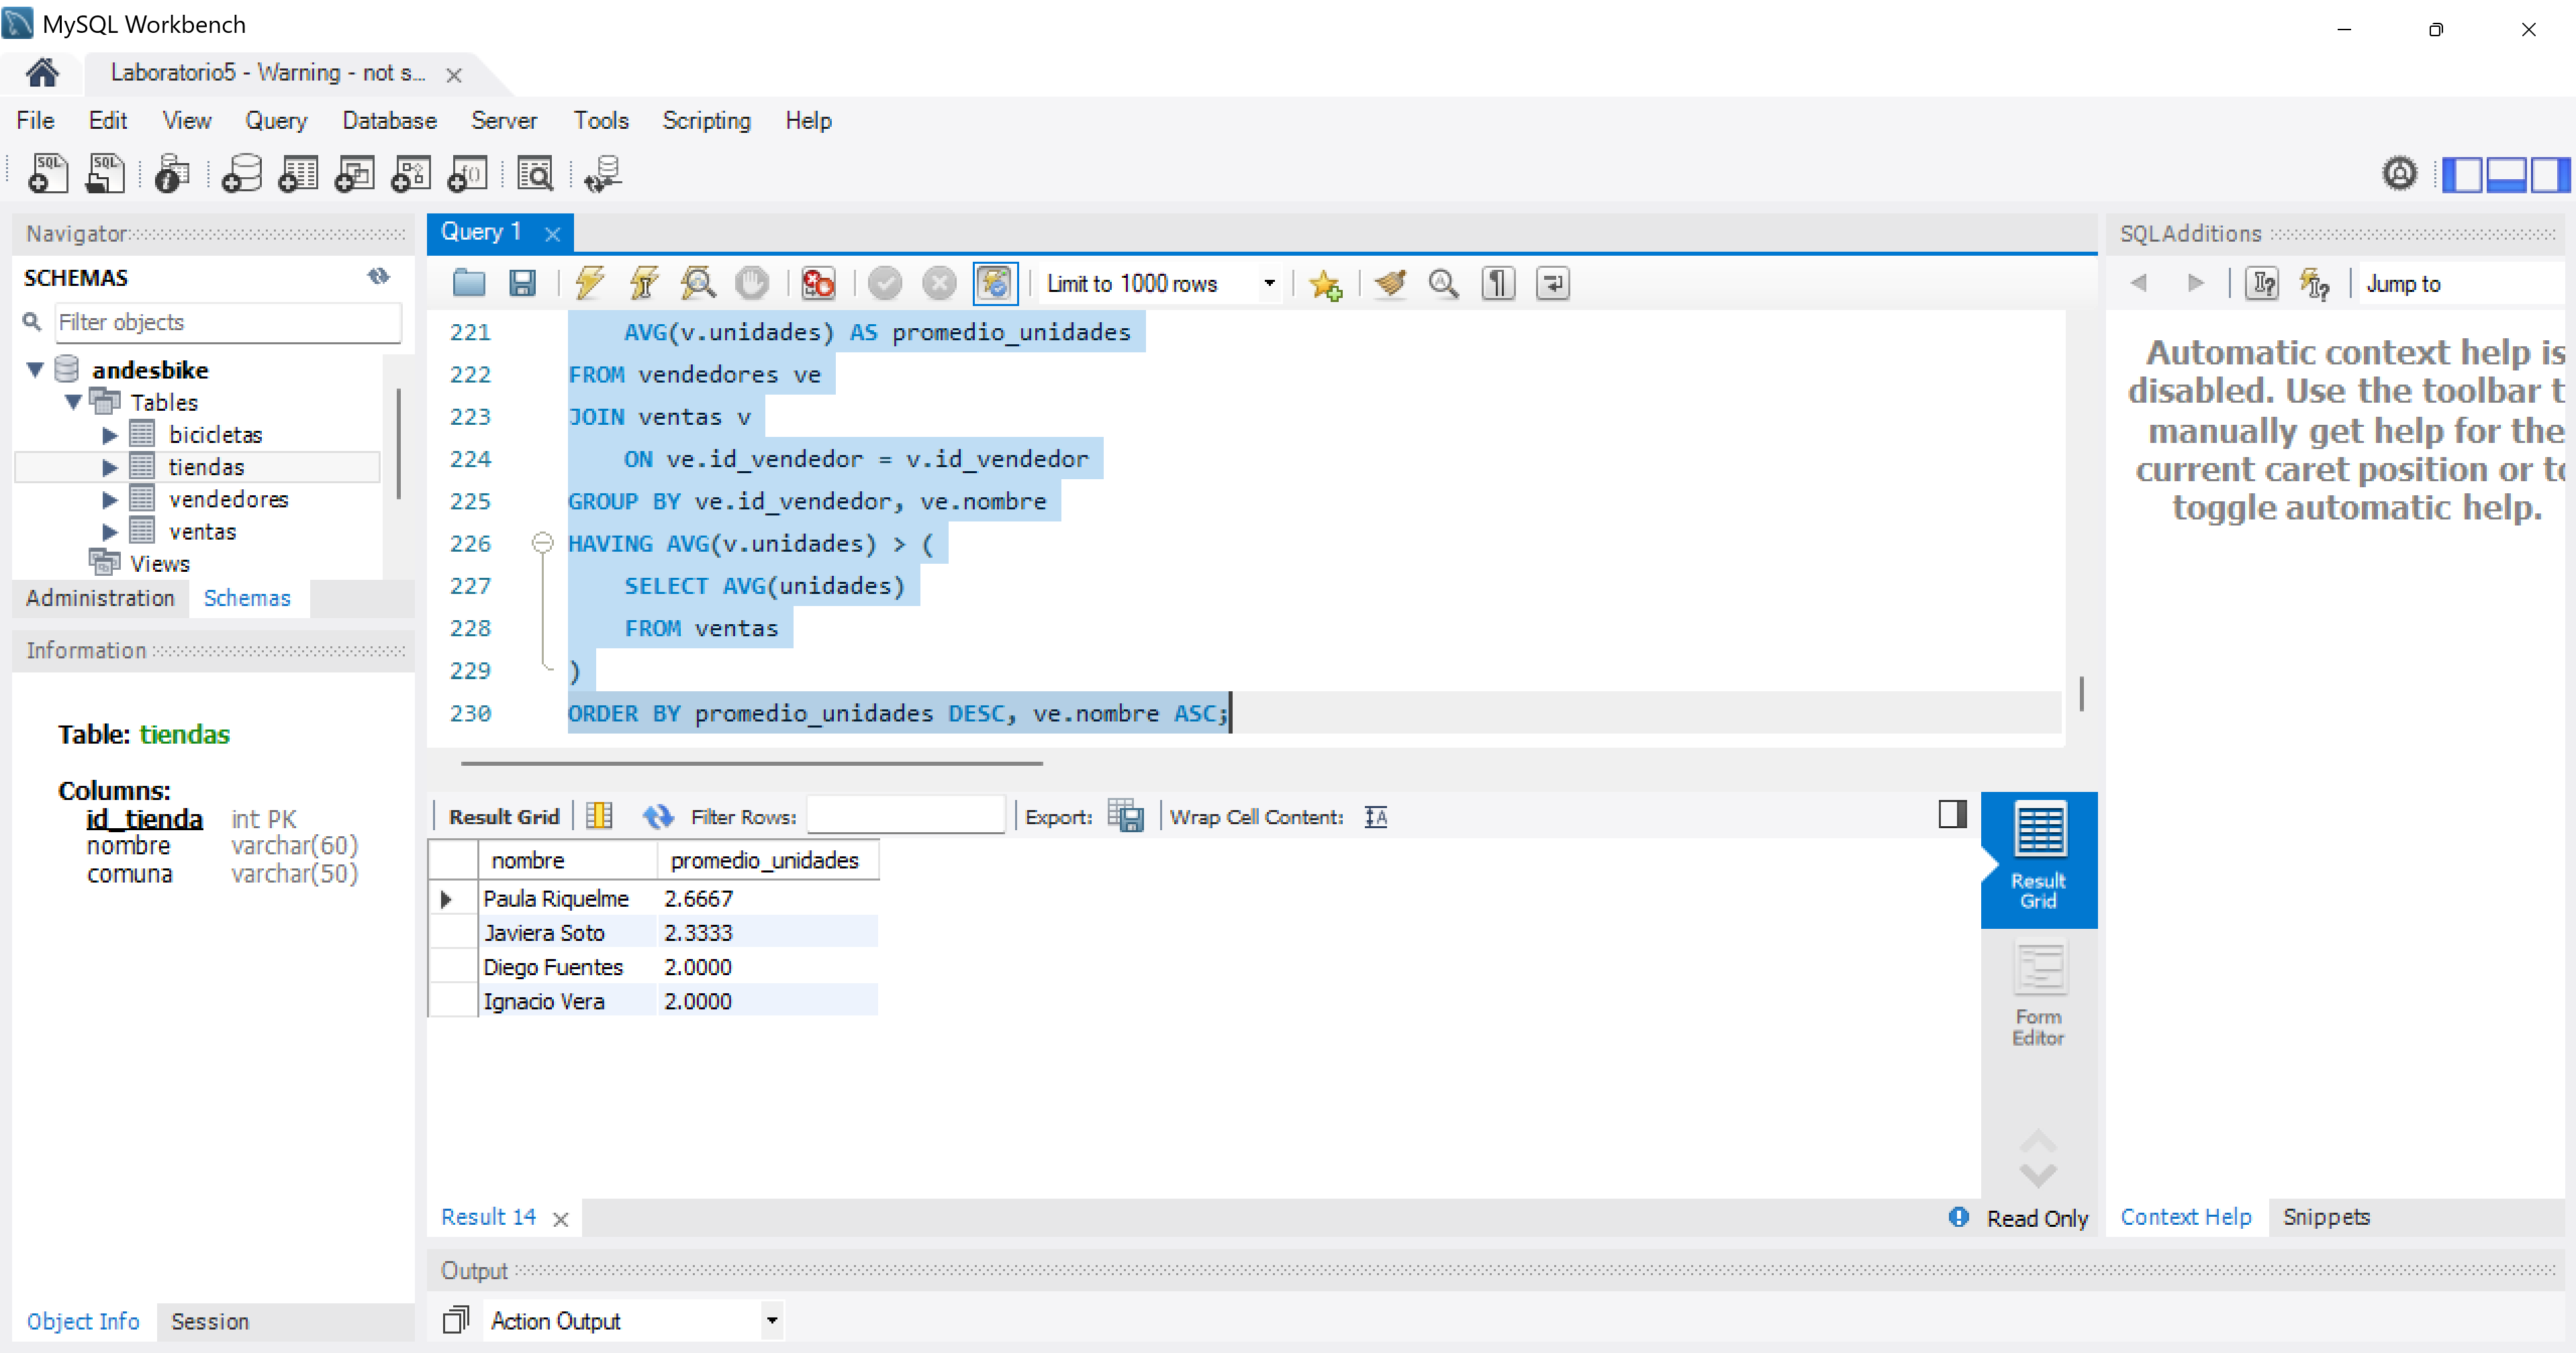
\includegraphics[width=0.95\textwidth,
height=0.38\textheight,keepaspectratio]{Consulta_09.png}
\end{figure}

\clearpage

\section*{Consulta 10}

\begin{lstlisting}[style=sqlstyle]
SELECT ve.nombre AS vendedor,
       SUM(v.unidades * b.precio) AS monto_total
FROM vendedores ve
LEFT JOIN ventas v
    ON ve.id_vendedor = v.id_vendedor
LEFT JOIN bicicletas b
    ON v.id_bicicleta = b.id_bicicleta
GROUP BY ve.id_vendedor, ve.nombre
ORDER BY monto_total DESC, ve.nombre ASC;
\end{lstlisting}

\noindent
Los vendedores sin ventas no muestran
cero porque la función \texttt{SUM()} devuelve \texttt{NULL}
cuando no existen registros asociados. Para que mostraran
cero, habría que agregar \texttt{COALESCE(SUM(...), 0)}.

\begin{figure}[H]
\centering
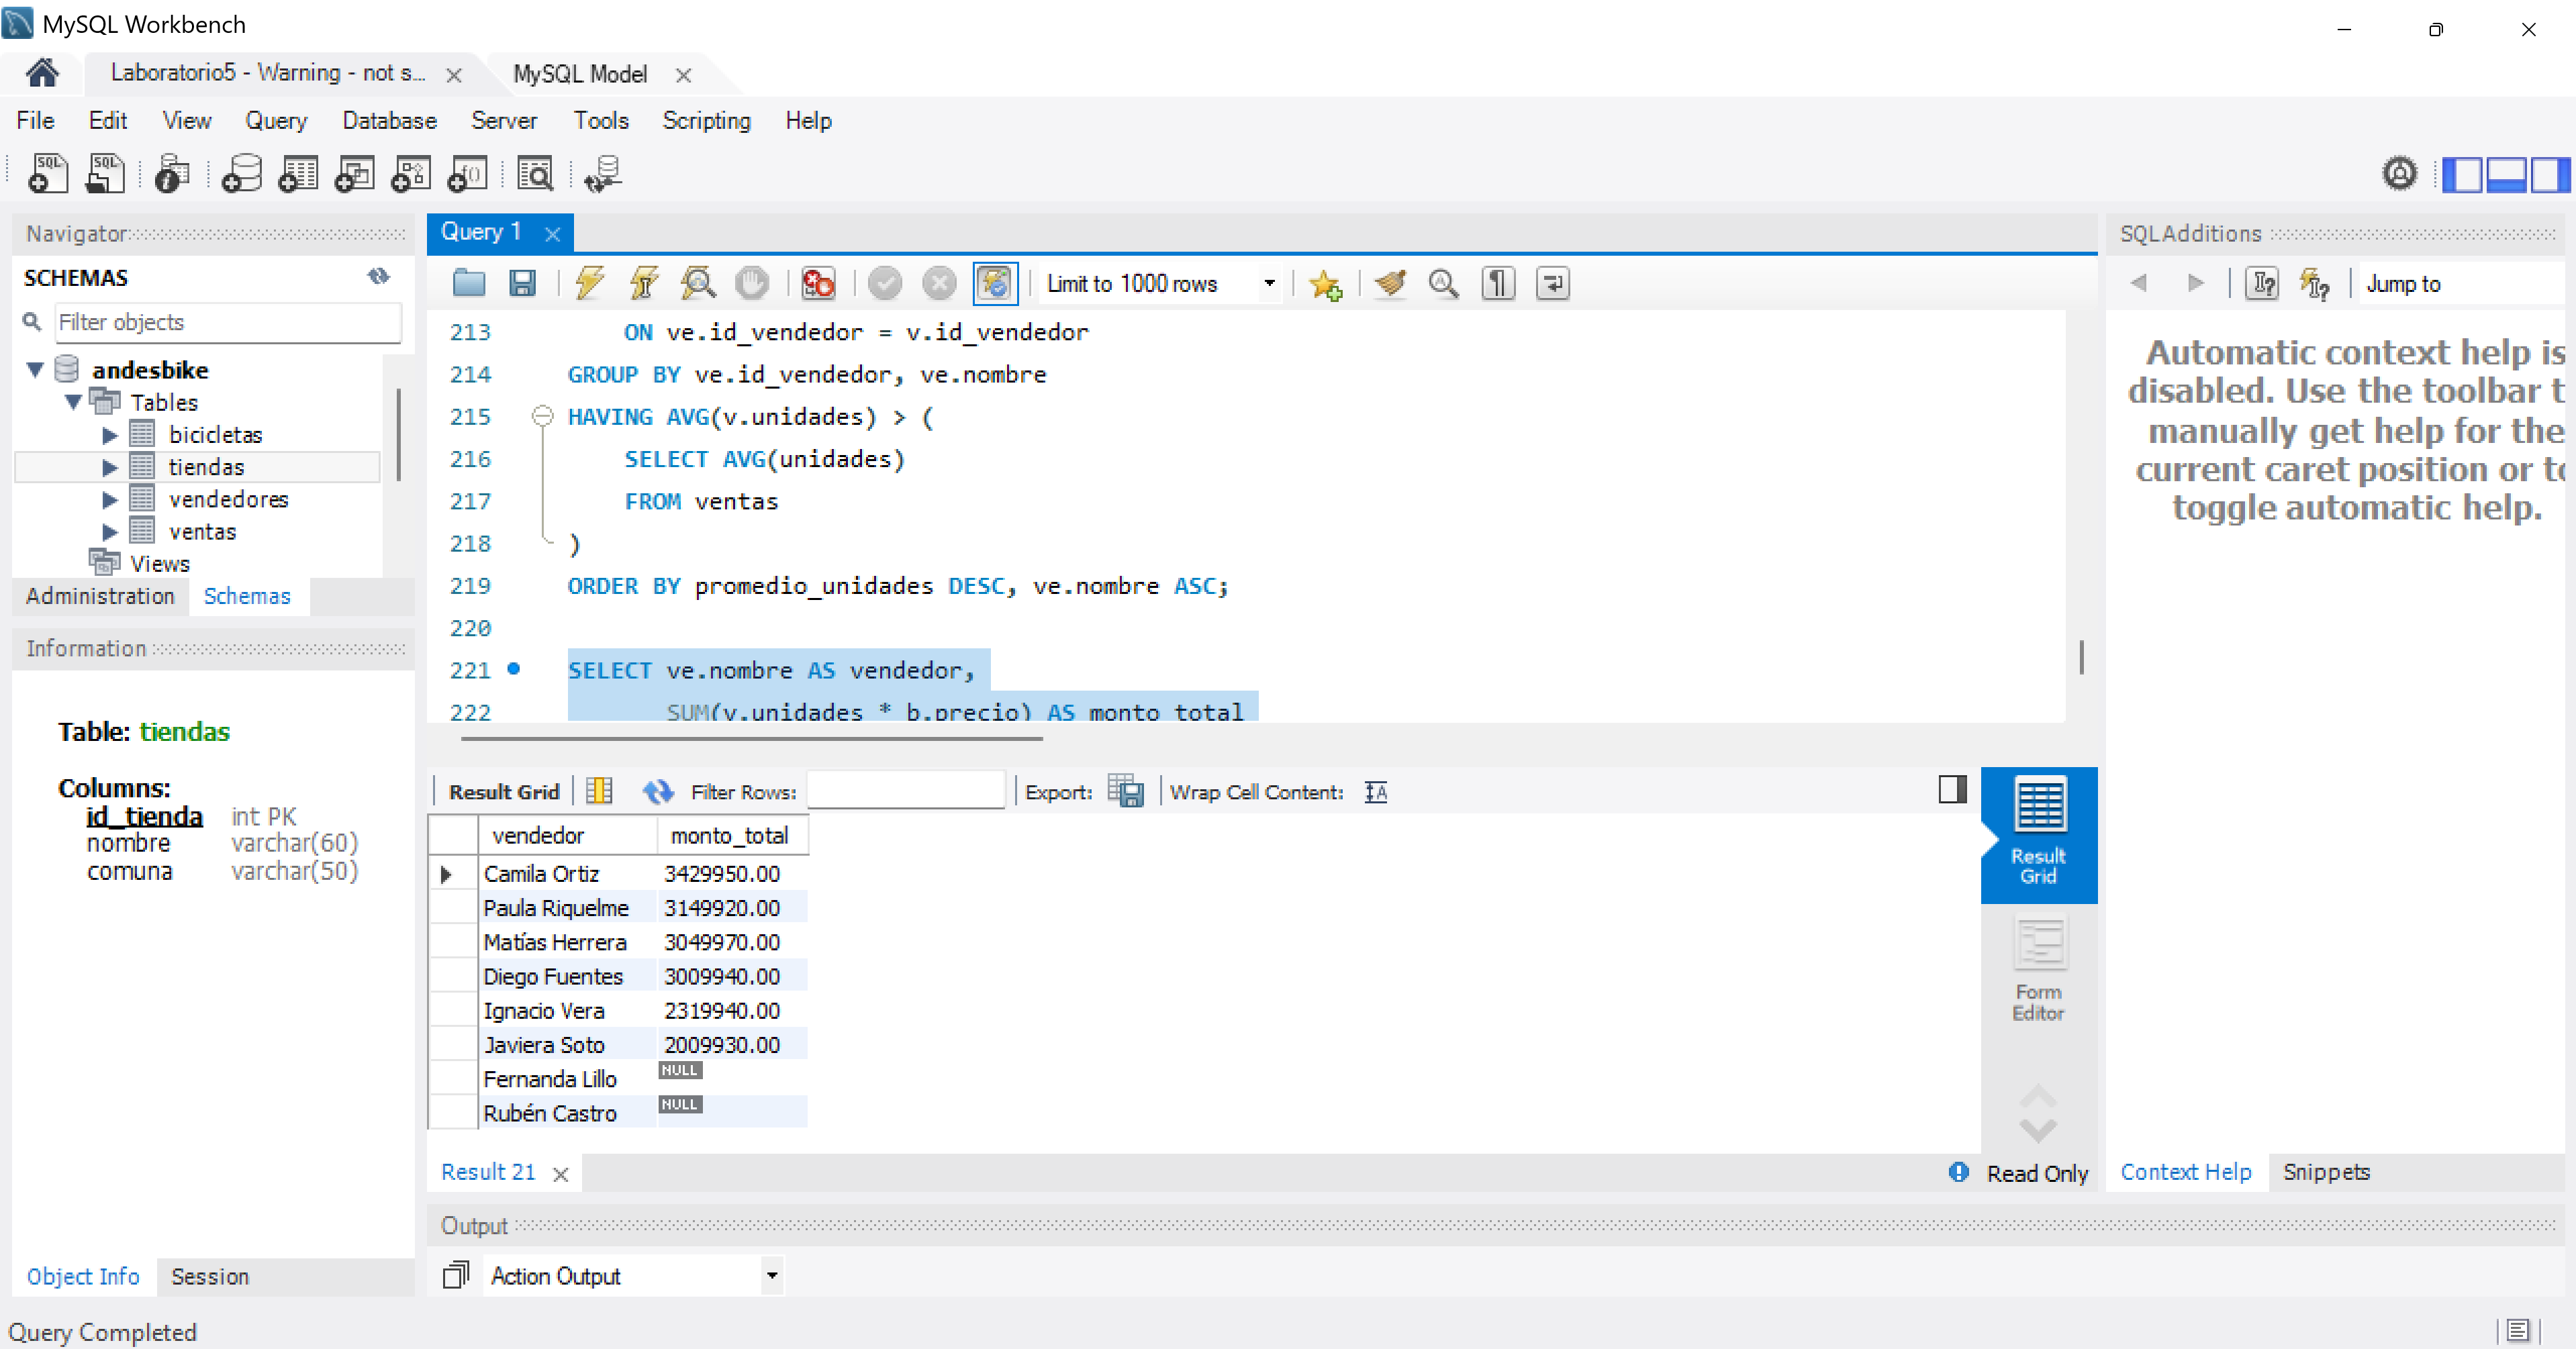
\includegraphics[width=0.95\textwidth,
height=0.38\textheight,keepaspectratio]{Consulta_10.png}
\end{figure}

\end{document}
